\chapterimage{chap33.jpg}
\chapter{July}
\section{Week \Rmnum{1}}
\textcolor{orange}{July 1}

\begin{example}[][Exam: 33.1.1]
	$$\lim\limits_{x\to +\infty}\left[ \dfrac{\ln(x+\sqrt{x^2+1})}{\ln(x+\sqrt{x^2-1})}\right]^{x^2\ln x}$$
\end{example}

\begin{solution}
	
	原极限等价于: 
	\begin{eqnarray*}
		I&=&\lim\limits_{x\to+\infty}e^{x^2\ln x\ln\left[1+\dfrac{\ln(x+\sqrt{x^2+1})-\ln(x+\sqrt{x^2-1})}{\ln(x+\sqrt{x^2-1})} \right] }\\
		I_{1}&=&\lim\limits_{x\to+\infty}x^2\ln x\ln\left[1+\dfrac{\ln(x+\sqrt{x^2+1})-\ln(x+\sqrt{x^2-1})}{\ln(x+\sqrt{x^2-1})} \right] \\
		&=&\lim\limits_{x\to+\infty}x^2\ln x(\dfrac{\ln(x+\sqrt{x^2+1})-\ln(x+\sqrt{x^2-1})}{\ln(x+\sqrt{x^2-1})})\\
		&=&\lim\limits_{x\to+\infty}x^2\ln x(\dfrac{(\sqrt{x^2+1}-\sqrt{x^2-1})}{\xi \ln(2x)}), \xi\in(x+\sqrt{x^2-1},x+\sqrt{x^2+1})\\
		&=&\lim\limits_{x\to+\infty}\dfrac{x}{\xi}\dfrac{2x}{(\sqrt{x^2+1}+\sqrt{x^2-1})}\\
		&=&\lim\limits_{x\to+\infty}\dfrac{x}{\xi}
	\end{eqnarray*}
	
	我们用夹逼定理: $\lim\limits_{x\to+\infty}\dfrac{x}{\xi}=\dfrac{1}{2}$
	
	原极限$I=e^{\dfrac{1}{2}}$
\end{solution}

\begin{example}[][Exam: 33.1.2]
	设 $f(x)$ 在 $[0,1]$ 导函数连续, 且 $\int_{0}^{1}x^2f'(x)dx=1$, 证明: 

(1). $\exists \xi\in(0,1),\ s.t. f'(\xi)=3$

(2). $f(1)=\int_{0}^{1}f(x)dx = 0 \to \exists \eta\in(0,1), \ s.t.\ f'(\eta)=-\dfrac{6}{7}$
\end{example}

\begin{solution}
	
	(1).我们不妨设$g(x)=x^2$,我们有$x\in(0,1),g(x)>0$,我们根据第一积分中值定理得到: 
	$$\exists\xi\in(0,1),\ s.t. \int_{0}^{1}f'(x)g(x)dx=f'(\xi)\int_{0}^{1}g(x)dx\Rightarrow \int_{}^{}x^2f'(x)dx=f'(\xi)\int_{0}^{1}x^2dx=\dfrac{1}{3}f'(\xi)=1$$
	
	综上所述,我们得到: $\exists \xi\in(0,1),\ s.t. f'(\xi)=3$
	
	(2).我们由$\int_{0}^{1}x^2f'(x)dx=1$得到: 
	$$\int_{0}^{1}f(x)dx=xf(x)|_{x=0}^{x=1}-\int_{0}^{1}xf'(x)dx=0\Rightarrow \int_{0}^{1}xf'(x)dx=0$$
	
	我们得到: 
	$$\left\lbrace
	\begin{array}{l}
		\int_{0}^{1}xf'(x)dx=0\\
		\int_{0}^{1}x^2f'(x)dx=1
	\end{array}
	\right. \Rightarrow \int_{0}^{1}(x^2-kx)f'(x)dx=1$$
	
	我们假设$h(x)=x^2-kx$,我们不妨假设$h(x)$在$(0,1)$上恒有$h(x)>0$或者$h(x)<0$,我们由第一积分中值定理得到: 
	$$\exists\eta\in(0,1),\ s.t. \int_{0}^{1}h(x)f'(x)=f'(\eta)\int_{0}^{1}h(x)dx\Rightarrow f'(\eta)\int_{0}^{1}(x^2-kx)dx=1\Rightarrow f'(\eta)=\dfrac{6}{2-3k}$$
	
	当$k=3$时,我们有$h(x)=x^2-3x$,当$x\in(0,1)$,$h(x)<0$,满足第一积分中值定理使用条件,我们可以得到: $\exists \eta\in(0,1), \ s.t. f'(\eta)=-\dfrac{6}{7}$
\end{solution}


\textcolor{orange}{July 2}

\begin{example}[][Exam: 33.1.3]
	设 $f(x)$ 连续, $\lim\limits_{x\to 0}\dfrac{f(x)}{x}=1$
	$$\lim\limits_{x\to 0 }\left[ 1+\int_{0}^{x}tf(x^2-t^2)dt\right]^{\frac{1}{(\tan x-x)\ln(1+x)}}$$
\end{example}
\begin{solution}
	
	原极限等价于: 
	\begin{eqnarray*}
		I&=&\lim\limits_{x\to 0}e^{\dfrac{3\int_{0}^{x^2}-\frac{1}{2}f(x^2-t^2)d(x^2-t^2)}{x^4}}\\
		&=&\lim\limits_{x\to 0}e^{\dfrac{\dfrac{3}{2}\int_{0}^{x^2}f(u)du}{x^4}}\\
		&=&\lim\limits_{x\to 0}e^{\dfrac{3f(x^2)}{4x^2}}\\
		&=&e^{\frac{3}{4}}
	\end{eqnarray*}
\end{solution}

\begin{example}[][Exam: 33.1.4]
	设 $f(x)$ 是 $(-\infty,+\infty)$ 上连续的周期为 $1$ 的周期函数且满足 $0\leq f(x)\leq 1, \int_{0}^{1}f(x)dx=1$,证明:
	$$x\in[0,13], \int_{0}^{\sqrt{x}}f(t)dt+\int_{0}^{\sqrt{x+27}}f(t)dt+\int_{0}^{\sqrt{13-x}}f(t)dt\leq 11$$
\end{example}
\begin{solution}
	
	我们由$0\leq f(x)\leq 1$得到: 
	$$\int_{0}^{\sqrt{x}}f(t)dt+\int_{0}^{\sqrt{x+27}}f(t)dt+\int_{0}^{\sqrt{13-x}}f(t)dt\leq \sqrt{x}+\sqrt{x+27}+\sqrt{13-x}=1\cdot\sqrt{x}+a\cdot\frac{1}{a}\sqrt{x+27}+b\cdot\frac{1}{b}\sqrt{13-x}$$
	
	我们由柯西不等式得到: 
	$$1\cdot\sqrt{x}+a\cdot\frac{1}{a}\sqrt{x+27}+b\cdot\frac{1}{b}\sqrt{13-x}\leq \sqrt{(1+a^2+b^2)(x+\dfrac{x+27}{a^2}+\dfrac{13-x}{b^2})}$$
	
	我们需要满足: 
	$$\left\lbrace
	\begin{array}{l}
		1+\dfrac{1}{a^2}-\dfrac{1}{b^2}=0\\
		(1+a^2+b^2)(\dfrac{27}{a^2}+\dfrac{13}{b^2})=121
	\end{array}
	\right. \Rightarrow \left\lbrace
	\begin{array}{l}
		a^2=2\\
		b^2=\dfrac{2}{3}
	\end{array}
	\right. $$
	
	我们可以得到原不等式取等号条件$\dfrac{\sqrt{x}}{1}=\dfrac{\sqrt{x+27}}{2}=\dfrac{3\sqrt{13-x}}{2}$,当且仅当$x=9$时等号成立.
	
	当$x=9$时,原不等式为: 
	$$\int_{0}^{3}f(t)dt+\int_{0}^{6}f(t)dt+\int_{0}^{2}f(t)dt=11\int_{0}^{1}f(t)dt=11$$
	
	综上所述,等号成立条件为$x=9$,原不等式成立.
\end{solution}


\textcolor{orange}{July 3}

\begin{example}[][Exam: 33.1.5]
	设 $D=\{(x,y)|0\leq x\leq 2,0\leq y\leq 2\}$, $f(x,y)$ 在 $D$ 上连续, $\iint\limits_{D}f(x,y)dxdy=0, \iint\limits_{D}xyf(x,y)dxdy=1$,证明: 
	$$\exists (\xi,\eta)\in D,\ s.t.\ \big|f'(\xi,\eta)\big|\geq \dfrac{2}{4\ln 2+3}$$
\end{example}
1. 
\begin{solution}
	
	我们由: $\iint\limits_{D}f(x,y)dxdy=0$,$\iint\limits_{D}xyf(x,y)dxdy=1$得到: 
	$$\iint\limits_{D}(xy-k)f(x,y)dxdy=1\Rightarrow \iint\limits_{D}|xy-k||f(x,y)|dxdy\geq 1$$
	
	我们由二重积分第一积分中值定理得到: 
	$$\exists (\xi,\eta)\in D, \ s.t. |f(\xi,\eta)|\iint\limits_{D}|xy-k|dxdy=\iint\limits_{D}|xy-k||f(x,y)|dxdy\geq 1$$
	
	我们得到: 
	$$\exists (\xi,\eta)\in D, \ s.t. |f(\xi,\eta)|\geq \dfrac{1}{\iint\limits_{D}|xy-k|dxdy}$$
	
	我们只需要找到$k$使得$\iint\limits_{D}|xy-k|dxdy=2\ln2+\dfrac{3}{2}$.
	\begin{figure}[htbp]
		\centering
		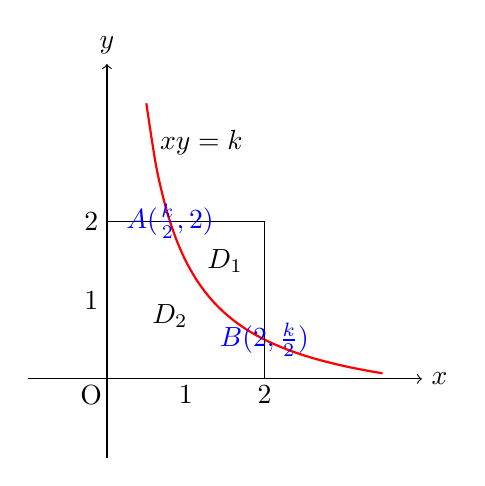
\begin{tikzpicture}
			\draw[->] (-1,0) -- (4,0) node[right] {$x$};
			\draw[->] (0,-1) -- (0,4) node[above] {$y$};
			\draw[red,thick, domain=0.5:3.5, smooth, variable=\x] plot ({\x},{2/\x-0.5});
			\draw(0,2) -- (2,2);
			\draw(2,0) -- (2,2);
			\node at (1,-0.2) {$1$};
			\node at (2,-0.2) {$2$};
			\node at (-0.2,1) {$1$};
			\node at (-0.2,2) {$2$};
			\node [blue] (A) at (0.8,2){$A(\frac{k}{2},2)$};
			\node [blue] (B) at (2,0.5){$B(2,\frac{k}{2})$};
			\node at (1.2,3) {$xy = k$}; 
			\node at (1.5,1.5) {$D_{1}$};
			\node at (0.8,0.8) {$D_{2}$};
			\node at (-0.2,-0.2) {O};
		\end{tikzpicture}
		\caption{积分区域图}
	\end{figure} 
	
	原二重积分等价于: 
	\begin{eqnarray*}
		I&=&\iint\limits_{D_{1}}(xy-k)dxdy+\iint\limits_{D_{2}}(k-xy)dxdy\\
		&=&\int_{\frac{k}{2}}^{2}dx\int_{\frac{k}{x}}^{2}(xy-k)dy+\int_{0}^{\frac{k}{2}}dx\int_{0}^{2}(k-xy)dy+\int_{\frac{k}{2}}^{2}dx\int_{0}^{\frac{k}{x}}(k-xy)dy\\
		&=&\dfrac{3}{4}k^2-4k+4+\dfrac{3}{4}k^2+k^2\ln 2-k^2\ln \frac{k}{2}\\
		&=&2k^2\ln 2-k^2\ln k+\dfrac{3}{2}k^2+4-4k
	\end{eqnarray*}
	
	我们得到: 
	$$\left\lbrace
	\begin{array}{l}
		2k^2=2\\
		\ln k=0\\
		\dfrac{3}{2}k^2+4-4k=\dfrac{3}{2}
	\end{array}
	\right. \Rightarrow k=1$$
	
	综上所述,我们找到$k=1$使得上式成立,我们有: $\exists (\xi,\eta)\in D,\ s.t. |f'(\xi,\eta)|\geq \dfrac{2}{4\ln 2+3}$
\end{solution}

\begin{example}[][Exam: 33.1.6]
	$$\lim\limits_{x\to+\infty}(x^{\frac{1}{x}}-1)^{\frac{1}{\ln x}}$$
\end{example}

\begin{solution}
	
	原极限等价于: 
	\begin{eqnarray*}
		I&=&\lim\limits_{x\to+\infty}e^{\dfrac{\ln(e^{\frac{\ln x}{x}}-1)}{\ln x}}\\
		&\overset{L}{=}&\lim\limits_{x\to+\infty}e^{\dfrac{(1-\ln x)e^{\frac{\ln x}{x}}}{x(e^{\frac{\ln x}{x}}-1)}}\\
		&=&\lim\limits_{x\to+\infty}e^{\dfrac{(1-\ln x)e^{\frac{\ln x}{x}}}{\ln x}}\\
		&=&e^{-1}
	\end{eqnarray*}
	\begin{anymark}[注]
		\begin{itemize}
			\item 如果$f\sim g$,我们有$\ln f\sim \ln g$
		\end{itemize}
	\end{anymark}
\end{solution}


\textcolor{orange}{July 4}

\begin{example}[][Exam: 33.1.7]
	已知 $a_{n}=\sum\limits_{k=1}^{n}\dfrac{1}{k^2}, b_{n}=\sum\limits_{k=1}^{n}\dfrac{1}{(2k-1)^2}$,
	且 $\lim\limits_{n\to +\infty}a_{n}=\dfrac{\pi^2}{6}$

(1). 证明: $a_{2n}=\dfrac{1}{4}a_{n}+b_{n}(n=1,2,\cdots)$

(2). $\lim\limits_{n\to+\infty}n\left(\dfrac{b_{n}}{a_{n}}-\dfrac{3}{4}\right) $
\end{example}
\begin{solution}
	
	(1). 我们有: $$\dfrac{1}{4}a_{n}=\dfrac{1}{4}\sum\limits_{k=1}^{n}\dfrac{1}{k^2}=\sum\limits_{k=1}^{n}\dfrac{1}{(2k)^2}$$
	
	因此,我们有: 
	\begin{eqnarray*}
		\dfrac{1}{4}a_{n}+b_{n}&=&\sum\limits_{k=1}^{n}\dfrac{1}{(2k)^2}+\sum\limits_{k=1}^{n}\dfrac{1}{(2k-1)^2}\\
		&=&\sum\limits_{k=1}^{2n}\dfrac{1}{k^2}\\
		&=&a_{2n}
	\end{eqnarray*}
	
	(2).原极限等价于: 
	\begin{eqnarray*}
		I&=&\lim\limits_{n\to+\infty}n\left( \dfrac{a_{2n}-a_{n}}{a_{n}}\right)\\
		&=&\dfrac{\lim\limits_{n\to+\infty}n(a_{2n}-a_{n})}{\lim\limits_{n\to+\infty}a_{n}}\\
		&=&\dfrac{6}{\pi^2}\lim\limits_{n\to+\infty}n\left[ \dfrac{1}{(n+1)^2}+\dfrac{1}{(n+2)^2}+\cdots+\dfrac{1}{(n+k)^2}+\cdots+\dfrac{1}{(n+n)^2}\right]\\
		&=& \dfrac{6}{\pi^2}\lim\limits_{n\to+\infty}\sum\limits_{k=1}^{n}\dfrac{1}{(1+\frac{k}{n})^2}\\
		&=&\dfrac{6}{\pi^2}(-\dfrac{1}{1+x})|_{0}^{1}\\
		&=&\dfrac{3}{\pi^2}
	\end{eqnarray*}
\end{solution}
\begin{anymark}[注]
	\begin{itemize}
		\item $\sum\limits_{n=1}^{+\infty}\dfrac{1}{n^2}=\dfrac{\pi^2}{6}$
		\item $\sum\limits_{n=1}^{+\infty}\dfrac{1}{(2n-1)^2}=\dfrac{\pi^2}{8}$
		\item $\sum\limits_{n=1}^{+\infty}\dfrac{1}{(2n)^2}=\dfrac{\pi^2}{24}$
	\end{itemize}
\end{anymark}

\begin{example}[][Exam: 33.1.8]
	$\lim\limits_{x\to 0}\dfrac{\cos(xe^x)-e^{-\frac{x^2}{2}e^{2x}}}{x^{\alpha}} = \beta\neq0$, 求 $\alpha,\beta$
\end{example}

\begin{solution}
	
	原极限等价于: 
	\begin{eqnarray*}
		I&=&\lim\limits_{x\to 0}\dfrac{1-\frac{1}{2}x^2e^{2x}+\frac{1}{24}x^4e^{4x}-(1-\frac{1}{2}x^2e^{2x}+\frac{1}{8}x^4e^{4x})}{x^{\alpha}}\\
		&=&\lim\limits_{x\to 0}\dfrac{-\frac{1}{12}x^4e^{4x}}{x^{\alpha}}\\
		&=&\beta
	\end{eqnarray*}
	
	我们得到: $\alpha=4,\ \beta=-\dfrac{1}{12}$
\end{solution}


\textcolor{orange}{July 5}

\begin{example}[][Exam: 33.1.9]
	$$\int_{0}^{+\infty}\dfrac{\ln x}{x^2+a^2}dx(a>0)$$
\end{example}

\begin{solution}
	
	原积分等价于: 
	\begin{eqnarray*}
		I&=&\dfrac{1}{a}\int_{0}^{+\infty}\dfrac{\ln a+\ln \frac{x}{a}}{(\frac{x}{a})^2+1}d(\frac{x}{a})\\
		&=&\dfrac{1}{a}\int_{0}^{+\infty}\dfrac{\ln a+\ln u}{u^2+1}du\\
		&=&\dfrac{\ln a}{a}\int_{0}^{+\infty}\dfrac{1}{u^2+1}du+\dfrac{1}{a}\int_{0}^{+\infty}\dfrac{\ln u}{u^2+1}du\\
		&=&I_{1}+I_{2}\\
		I_{1}&=&\dfrac{\pi \ln a}{2a}\\
		I_{2}&=&\dfrac{1}{a}\int_{0}^{+\infty}\dfrac{\ln u}{u^2+1}du=\dfrac{1}{a}\int_{+\infty}^{0}\dfrac{-\ln t }{(\frac{1}{t})^2+1}(-\dfrac{1}{t^2})dt=-\dfrac{1}{a}\int_{0}^{+\infty}\dfrac{\ln t}{t^2+1}dt\Rightarrow I_{2}=0\\
		I&=&I_{1}+I_{2}=\dfrac{\pi \ln a}{2a}
	\end{eqnarray*}
\end{solution}
\begin{anymark}[$\int_{0}^{+\infty}f(x)dx$积分技巧]
	\begin{itemize}
		\item 倒代换
		\item 分割为$\int_{0}^{1}f(x)+\int_{1}^{+\infty}f(x)dx$
		\item 利用正切三角换元法
	\end{itemize}
\end{anymark}

\begin{example}[][Exam: 33.1.10]
	$\lim\limits_{x\to 0}\dfrac{\cos 2x-\cos x\sqrt{\cos 2x}}{x^{\alpha}}=\beta\neq0$, 求 $\alpha,\beta$
\end{example}

\begin{solution}
	
	原极限等价于: 
	\begin{eqnarray*}
		I&=&\lim\limits_{x\to 0}\dfrac{\cos^2 2x-\cos^2 x\cos 2x}{(\cos x+\cos x\sqrt{\cos 2x})x^{\alpha}}\\
		&=&\lim\limits_{x\to 0}\dfrac{-\cos2x\sin^2 x}{(\cos x+\cos x\sqrt{\cos 2x})x^{\alpha}}\\
		&=&\lim\limits_{x\to 0}\dfrac{-\cos 2x}{\cos x+\cos x\sqrt{\cos 2x}}\lim\limits_{x\to 0}\dfrac{\sin^2 x}{x^{\alpha}}\\
		&=&-\dfrac{1}{2}\lim\limits_{x\to 0}\dfrac{\sin^2 x}{x^{\alpha}}\\
		&=&\beta
	\end{eqnarray*}
	
	我们可以得到: $\alpha=2,\ \beta=-\dfrac{1}{2}$
\end{solution}


\textcolor{orange}{July 6}

\begin{example}[][Exam: 33.1.11]
	设 $f(x)=\dfrac{1}{1+3x+9x^2}$, 求 $f^{(100)}(0)$
\end{example}

\begin{solution}
	
	我们可以得到: 
	$$f(x)=\dfrac{1-3x}{(1-3x)(1+3x+9x^2)}=\dfrac{1}{1-(3x)^3}-3x\dfrac{1}{1-(3x)^3}$$
	
	我们将$f(x)$在$x=0$处泰勒展开得到: 
	$$\left\lbrace
	\begin{array}{l}
		f(x)=a_{0}+a_{1}x+a_{2}x^2+\cdots+a_{100}x^{100}+\cdots+a_{n}x^{n}+\cdots\\
		f(x)=f(0)+f'(0)x+\dfrac{f''(0)}{2!}x^2+\cdots+\dfrac{f^{(100)}}{100!}x^{100}+\cdots
	\end{array}
	\right. \Rightarrow f^{(100)}(0)=a_{100}100!$$
	
	我们有: $$-1<x<1,\ 1+x+x^2+x^3+\cdots+x^n=\dfrac{1}{1-x}$$
	
	我们得到: 
	$$f(x)=\sum\limits_{n=0}^{+\infty}(3x)^{3n}-\sum\limits_{n=0}^{+\infty}(3x)^{3n+1}$$
	
	我们得到: $a_{100}=-3^{100}\Rightarrow f^{(100)}(0)=-3^{100}100!$
\end{solution}

\begin{example}[][Exam: 33.1.12]
	$\lim\limits_{x\to 0}\dfrac{ax^2+bx+1-e^{x^2-2x}}{x^2}=2$, 求 $a,b$
\end{example}

\begin{solution}
	
	原极限等价于: 
	\begin{eqnarray*}
		I&=&\lim\limits_{x\to 0}\dfrac{ax^2+bx+1-(1+x^2-2x+\frac{1}{2}(x^2-2x)^2)}{x^2}\\
		&=&\lim\limits_{x\to 0}\dfrac{(b+2)x+(a-3)x^2}{x^2}\\
		&=&a-3
	\end{eqnarray*}
	
	我们得到: $\left\lbrace
	\begin{array}{l}
		a-3=2\\
		b+2=0
	\end{array}
	\right. \Rightarrow \left\lbrace
	\begin{array}{l}
		a=5\\
		b=-2
	\end{array}
	\right. $
\end{solution}


\textcolor{orange}{July 7}

\begin{example}[][Exam: 33.1.13]
	$$\lim\limits_{x\to 0}\dfrac{n!x^n-\sin x\sin 2x\cdots\sin nx}{x^{n+2}}$$
\end{example}

\begin{solution}
	
	原极限等价于: 
	\begin{eqnarray*}
		I&=&n!\lim\limits_{x\to 0}\dfrac{1-\frac{\sin x\sin 2x\cdots\sin nx}{n!x^n}}{x^2}\\
		&=&n!\lim\limits_{x\to 0}\dfrac{1-\frac{\sin x}{x}\frac{\sin 2x}{2x}\cdots\frac{\sin nx}{nx}}{x^2}\\
		&=&-n!\lim\limits_{x\to 0}\dfrac{\ln(\frac{\sin x}{x}\frac{\sin 2x}{2x}\cdots\frac{\sin nx}{nx})}{x^2}\\
		&=&-n!\sum\limits_{k=1}^{n}\lim\limits_{x\to 0}\dfrac{\ln(1+\frac{\sin kx-kx}{kx})}{x^2}\\
		&=&n!\sum\limits_{k=1}^{n}\lim\limits_{x\to 0}\dfrac{kx-\sin kx}{kx^3}\\
		&=&n!\sum\limits_{k=1}^{n}(\dfrac{k^2}{6})\\
		&=&n!\dfrac{n(n+1)(2n+1)}{36}\\
		&=&\dfrac{n(2n+1)(n+1)!}{36}
	\end{eqnarray*}
\end{solution}

\begin{example}[][Exam: 33.1.14]
	$\lim\limits_{x\to 0}\left(\dfrac{\ln(x+\sqrt{x^2+1})+ax^2+bx^3}{x} \right)^{\frac{1}{x^2}}=e^2$, 求 $a,b$
\end{example}
\begin{solution}
	
	原极限等价于: 
	\begin{eqnarray*}
		I&=&\lim\limits_{x\to 0}e^{\dfrac{\ln(\frac{\ln(x+\sqrt{1+x^2})+ax^2+bx^3-x}{x}+1)}{x^2}}\\
		&=&\lim\limits_{x\to 0}e^{\dfrac{\ln(x+\sqrt{1+x^2})+ax^2+bx^3-x}{x^3}}\\
		&=&e^{\lim\limits_{x\to 0}\dfrac{x-\frac{1}{6}x^3+o(x^3)+ax^2+bx^3-x}{x^3}}\\
		&=&e^{\lim\limits_{x\to 0}\dfrac{(b-\frac{1}{6})x^3+o(x^3)+ax^2}{x^3}}\\
		&=&e^2
	\end{eqnarray*}
	
	我们得到: $\left\lbrace
	\begin{array}{l}
		b-\frac{1}{6}=2\\
		a=0
	\end{array}
	\right. \Rightarrow \left\lbrace
	\begin{array}{l}
		b=\dfrac{13}{6}\\
		a=0
	\end{array}
	\right. $
\end{solution}
\begin{anymark}[注]
	$x\to 0,\ x\sim \ln(x+\sqrt{x^2+1})$
	
	我们可以得到: 
	$$[\ln(x+\sqrt{x^2+1})]'=\dfrac{1}{\sqrt{1+x^2}}=(1+x^2)^{\frac{1}{2}}=1-\dfrac{1}{2}x^2+\dfrac{3}{8}x^3+\cdots$$
	
	我们可以得到: $\ln(x+\sqrt{1+x^2})$的泰勒展开式: 
	$$\ln(x+\sqrt{1+x^2})=x-\dfrac{1}{6}x^3+o(x^3)$$
\end{anymark}


\section{Week \Rmnum{2}}

\textcolor{blue}{July 8}

\begin{example}[][Exam: 33.2.1]
	设 $n$ 阶矩阵 $A,B$ 满足 $AB+aA+bB+cE=O$, 其中 $ab\neq c$, 证明: 

(1). $A+bE$ 与 $B+aE$ 均为可逆矩阵 

(2). $AB=BA$
\end{example}
1. 

\begin{solution}
	
	(1). 我们由$AB+aA+bB+cE=O$可以得到: 
	$$(A+bE)(B+aE)=(ab-c)E$$
	
	我们得到: $$\left\lbrace
	\begin{array}{l}
		\dfrac{1}{ab-c}(A+bE)(B+aE)=E\\
		(A+bE)\dfrac{1}{ab-c}(B+aE)=E
	\end{array}
	\right. $$
	
	我们得到: $A+bE$与$B+aE$均为可逆矩阵 
	
	(2). 我们可以得到: 
	$$\dfrac{1}{ab-c}(A+bE)(B+aE)=\dfrac{1}{ab-c}(B+aE)(A+bE)$$
	
	我们化简一下: 
	$$\left\lbrace
	\begin{array}{l}
		\text{左边}=AB+bB+aA+abE\\
		\text{右边}=BA+aA+bB+abE
	\end{array}
	\right. \Rightarrow AB=BA$$
\end{solution}

\begin{example}[][Exam: 33.2.2]
	已知常数 $a>0, bc\neq 0$, 且 $\lim\limits_{x\to+\infty}[x^a\ln(1+\frac{x}{b})-x]=c$, 求 $a,b,c$
\end{example}

\begin{solution}
	
	原极限等价于: 
	\begin{eqnarray*}
		I&=&\lim\limits_{x\to 0 }\dfrac{\ln(1+bx)-x^{a-1}}{x^a}\\
		&=&\lim\limits_{x\to 0 }\dfrac{bx-\frac{1}{2}b^2x^2-x^{a-1}}{x^a}\\
		&=&c
	\end{eqnarray*}
	
	我们得到: $\left\lbrace
	\begin{array}{l}
		a-1=1\\
		b=1\\
		c=-\dfrac{1}{2}b^2
	\end{array}
	\right. \Rightarrow \left\lbrace
	\begin{array}{l}
		a=2\\
		b=1\\
		c=-\dfrac{1}{2}
	\end{array}
	\right. $
\end{solution}


\textcolor{blue}{July 9}

\begin{example}[][Exam: 33.2.3]
	$$\lim\limits_{n\to +\infty}\dfrac{1}{n}\left[\int_{\frac{1}{3}}^{\frac{1}{6n}}\dfrac{\sin y}{y}dy+\int_{\frac{1}{3}}^{\frac{3}{6n}}\dfrac{\sin y}{y}dy+\cdots+\int_{\frac{1}{3}}^{\frac{(2n-1)}{6n}}\dfrac{\sin y}{y}dy \right]$$
\end{example}

\begin{solution}
	
	原极限等价于: 
	\begin{eqnarray*}
		I&=&\lim\limits_{n\to +\infty}\dfrac{1}{n}\sum\limits_{k=1}^{n}\int_{\frac{1}{3}}^{\frac{2k-1}{6n}}\dfrac{\sin y}{y}dy\\
		&=&\lim\limits_{n\to +\infty}\dfrac{1}{n}\sum\limits_{k=1}^{n}f(\frac{2k-1}{2n})\\
		&=&\int_{0}^{1}[\int_{\frac{1}{3}}^{\frac{1}{3}x}\dfrac{\sin y}{y}dy]dx\\
		&=&-\int_{0}^{\frac{1}{3}}dy\int_{0}^{3y}\dfrac{\sin y}{y}dx\\
		&=&-\int_{0}^{\frac{1}{3}}3\sin ydy\\
		&=&3(\cos \frac{1}{3}-1)
	\end{eqnarray*}
\end{solution}

\begin{example}[][Exam: 33.2.4]
	设 $A$ 为 $n$ 阶反对称矩阵, 证明: 对于任意向量 $x$, 均有 $x^{T}(A+E)x\geq 0$
\end{example}

\begin{solution}
	
	我们有: $$x^{T}(A+E)x=[x^{T}(A+E)x]^T=x^{T}(A^{T}+E)x=x^{T}(-A+E)x$$
	
	$$x^{T}(A+E)x+x^{T}(A-E)x=2x^{T}Ax=0\Rightarrow x^{T}(A+E)x=x^{T}Ax+x^{T}Ex=x^{T}x\geq 0$$
\end{solution}


\textcolor{blue}{July 10}

\begin{example}[][Exam: 33.2.5]
	$$\dfrac{n^{s+1}}{s+1} < 1^s+2^s+\cdots+n^s < \dfrac{(n+1)^{s+1}}{s+1} (s > 0)$$
\end{example}

\begin{figure}[H]
	\centering
	\subfigure[定积分定义示意图$\alpha$]{
		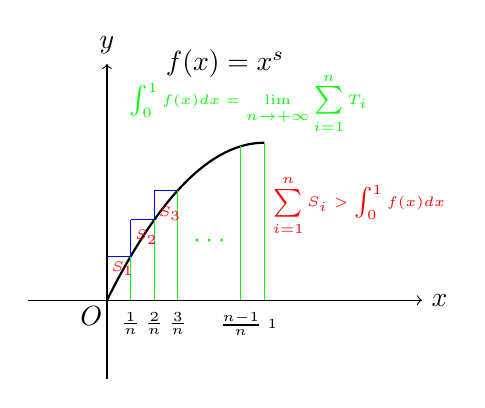
\begin{tikzpicture}
			\draw[->] (-1,0) -- (4,0) node[right] {$x$};
			\draw[->] (0,-1) -- (0,3) node[above] {$y$};
			\draw[thick, domain=0:2, smooth, variable=\x] plot ({\x},{-0.5*\x*\x+2*\x});
			\draw[green] (0.3,0) -- (0.3,0.555);
			\draw[green] (0.6,0) -- (0.6,1.02);
			\draw[green] (0.9,0) -- (0.9,1.395);
			\draw[green] (1.7,0) -- (1.7,1.955);
			\draw[green] (2,0) -- (2,2);
			\draw[blue] (0,0.555) -- (0.3,0.555);
			\draw[blue] (0.3,0.555) -- (0.3,1.02);
			\draw[blue] (0.3,1.02) -- (0.6,1.02);
			\draw[blue] (0.6,1.02) -- (0.6,1.395);
			\draw[blue] (0.6,1.395) -- (0.9,1.395);
			\node[green] at (1.3,0.75) {$\cdots$};
			\node at (0.3,-0.3) {\tiny{$\frac{1}{n}$}};
			\node at (0.6,-0.3) {\tiny{$\frac{2}{n}$}};
			\node at (0.9,-0.3) {\tiny{$\frac{3}{n}$}};
			\node at (1.7,-0.3) {\tiny{$\frac{n-1}{n}$}};
			\node at (2.1,-0.3) {\tiny{$1$}};
			\node at (-0.2,-0.2) {$O$};
			\node at (1.5,3) {$f(x) = x^{s}$};
			\node[red] at (0.2,0.4) {\tiny{$S_{1}$}};
			\node[red] at (0.5,0.8) {\tiny{$S_{2}$}};
			\node[red] at (0.8,1.1) {\tiny{$S_{3}$}};
			\node[green] at (1.8,2.5) {\tiny{$\int_{0}^{1}f(x) dx=\lim\limits_{n\to +\infty}\sum\limits_{i=1}^{n}T_{i}$}};
			\node[red] at (3.2,1.2) {\tiny{$\sum\limits_{i=1}^{n}S_{i} > \int_{0}^{1}f(x)dx$}};
		\end{tikzpicture}	
	}
	\subfigure[定积分定义示意图$\beta$]{
		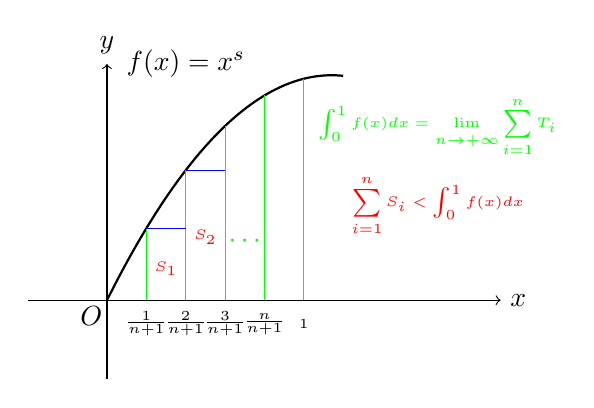
\begin{tikzpicture}
			\draw[->] (-1,0) -- (5,0) node[right] {$x$};
			\draw[->] (0,-1) -- (0,3) node[above] {$y$};
			\draw[thick, domain=0:3, smooth, variable=\x] plot ({\x},{-0.35*\x*\x+2*\x});
			\draw[green] (0.5,0) -- (0.5,0.9125);
			\draw[green] (1,0) -- (1,1.65);
			\draw[green] (1.5,0) -- (1.5,2.2125);
			\draw[green] (2,0) -- (2,2.6);
			\draw[green] (2.5,0) -- (2.5,2.8125);
			\draw[blue] (0.5,0.9125) -- (1,0.9125);
			\draw[blue] (1,1.65) -- (1.5,1.65);
			\node[green] at (1.75,0.75) {$\cdots$};
			\node at (0.5,-0.3) {\tiny{$\frac{1}{n+1}$}};
			\node at (1,-0.3) {\tiny{$\frac{2}{n+1}$}};
			\node at (1.5,-0.3) {\tiny{$\frac{3}{n+1}$}};
			\node at (2,-0.3) {\tiny{$\frac{n}{n+1}$}};
			\node at (2.5,-0.3) {\tiny{$1$}};
			\node at (-0.2,-0.2) {$O$};
			\node at (1,3) {$f(x) = x^{s}$};
			\node[red] at (0.75,0.4) {\tiny{$S_{1}$}};
			\node[red] at (1.25,0.8) {\tiny{$S_{2}$}};
			\node[green] at (4.2,2.2) {\tiny{$\int_{0}^{1}f(x) dx=\lim\limits_{n\to +\infty}\sum\limits_{i=1}^{n}T_{i}$}};
			\node[red] at (4.2,1.2) {\tiny{$\sum\limits_{i=1}^{n}S_{i} < \int_{0}^{1}f(x)dx$}};
		\end{tikzpicture}
		}
	\caption{积分和求和关系图}
\end{figure} 
\begin{solution}
	
	原不等式可以化为: 
	$$\left\lbrace
	\begin{array}{l}
		\dfrac{1}{n}[(\frac{1}{n})^s+(\frac{2}{n})^s+\cdots+(\frac{n}{n})^s]>\dfrac{1}{s+1}\\
		\dfrac{1}{n+1}[(\frac{1}{n+1})^s+(\frac{2}{n+1})^s+\cdots+(\frac{n}{n+1})^s]<\dfrac{1}{s+1}
	\end{array}
	\right. $$
	
	如图$(a)$第一个不等式: 
	$$\text{左边}=\sum\limits_{i=1}^{n}S_{i}>\int_{0}^{1}x^sdx=\dfrac{1}{s+1}=\text{右边}$$
	
	如图$(b)$第二个不等式: 
	$$\text{左边}=\sum\limits_{i=1}^{n}S_{i}<\int_{0}^{1}x^sdx=\dfrac{1}{s+1}=\text{右边}$$
\end{solution}

\begin{example}[][Exam: 33.2.6]
	$$\lim\limits_{n\to +\infty}\dfrac{1^{p+1}+2^{p+1}+\cdots+n^{p+1}}{n(1^p+2^p+\cdots+n^p)}(p>0)$$
\end{example}

\begin{solution}
	
	原极限等价于: 
	\begin{eqnarray*}
		I&=&\lim\limits_{n\to +\infty}\dfrac{(\frac{1}{n})^{p+1}+(\frac{2}{n})^{p+1}+\cdots+(\frac{n}{n})^{p+1}}{(\frac{1}{n})^{p}+(\frac{2}{n})^{p}+\cdots+(\frac{n}{n})^{p}}\\
		&=&\lim\limits_{n\to +\infty}\dfrac{\frac{1}{n}[(\frac{1}{n})^{p+1}+(\frac{2}{n})^{p+1}+\cdots+(\frac{n}{n})^{p+1}]}{\frac{1}{n}[(\frac{1}{n})^{p}+(\frac{2}{n})^{p}+\cdots+(\frac{n}{n})^{p}]}\\
		&=&\lim\limits_{n\to +\infty}\dfrac{\frac{1}{n}\sum\limits_{k=1}^{n}(\frac{k}{n})^{p+1}}{\frac{1}{n}\sum\limits_{k=1}^{n}(\frac{k}{n})^{p}}\\
		&=&\dfrac{\int_{0}^{1}\dfrac{x^{p+2}}{p+2}dx}{\int_{0}^{1}\dfrac{x^{p+1}}{p+1}dx}\\
		&=&\dfrac{p+1}{p+2}
	\end{eqnarray*}
\end{solution}


\textcolor{blue}{July 11}

\begin{example}[][Exam: 33.2.7]
	已知 $ A = 
	\begin{bmatrix}
		0 & -1 & 1\\
		2 & -3 & 0\\
		0 &  0 & 0
	\end{bmatrix}$, 求 $A^{99}$
\end{example}

\begin{solution}
	
	我们将矩阵$A$相似对角化: 
	
	(1). 求矩阵$A$的特征值和特征向量
	
	$$\left| \lambda E-A\right|=\left| \begin{matrix}
		\lambda&1&-1\\-2&\lambda+3&0\\
		0&0&\lambda
	\end{matrix}\right|=\lambda(\lambda+1)(\lambda+2)$$
	
	矩阵$A$的特征值为$\lambda_{1}=0,\ \lambda_{2}=-1,\ \lambda_{3}=-2$
	
	当$\lambda_{1}=0$时,$(-A)x=0\Rightarrow \left[ \begin{matrix}
		0&1&-1\\
		-2&3&0\\
		0&0&0
	\end{matrix}\right]\left[ \begin{matrix}
		x_{1}\\x_{2}\\x_{3}
	\end{matrix}\right]=0\Rightarrow \xi_{1}=(3,2,2)^T$
	
	当$\lambda_{2}=-1$时,$(-E-A)x=0\Rightarrow \left[ \begin{matrix}
		-1&1&-1\\
		-2&2&0\\
		0&0&-1
	\end{matrix}\right]\left[ \begin{matrix}
		x_{1}\\x_{2}\\x_{3}
	\end{matrix}\right]=0\Rightarrow \xi_{2}=(1,1,0)^T$
	
	当$\lambda_{3}=-2$时,$(-2E-A)x=0\Rightarrow \left[ \begin{matrix}
		-2&1&-1\\
		-2&1&0\\
		0&0&-2
	\end{matrix}\right]\left[ \begin{matrix}
		x_{1}\\x_{2}\\x_{3}
	\end{matrix}\right]=0\Rightarrow \xi_{3}=(1,2,0)^T$
	
	存在可逆矩阵$P=\left[ \begin{matrix}
		3&1&1\\2&1&2\\2&0&0
	\end{matrix}\right]$,$\ s.t. \ P^{-1}AP=\varLambda=\left[ \begin{matrix}
		0& & \\ &-1& \\ & &-2
	\end{matrix}\right]$,其中$P^{-1}=\left[ \begin{matrix}
		0&0&\frac{1}{2}\\2&-1&-2\\-1&1&\frac{1}{2}
	\end{matrix}\right]$
	
	我们得到: $$A=P\varLambda P^{-1}\Rightarrow A^{99}=P\varLambda^{99}P^{-1}$$
	
	上面的式子可以化为: 
	\begin{eqnarray*}
		A^{99}&=&\left[ \begin{matrix}
			3&1&1\\2&1&2\\2&0&0
		\end{matrix}\right]\left[ \begin{matrix}
			0& & \\ &-1& \\ & &-2^{99}
		\end{matrix}\right]\left[ \begin{matrix}
			0&0&\frac{1}{2}\\2&-1&-2\\-1&1&\frac{1}{2}
		\end{matrix}\right]\\
		&=&\left[ \begin{matrix}
			0&-1&-2^{99}\\0&-1&-2^{100}\\0&0&0
		\end{matrix}\right]\left[ \begin{matrix}
			0&0&\frac{1}{2}\\2&-1&-2\\-1&1&\frac{1}{2}
		\end{matrix}\right]\\
		&=&\left[ \begin{matrix}
			2^{99}-2&1-2^{99}&2-2^{98}\\2^{100}-2&1-2^{100}&2-2^{99}\\0&0&0
		\end{matrix}\right]
	\end{eqnarray*}
\end{solution}

\begin{example}[][Exam: 33.2.8]
	设 $3$ 阶实对称矩阵 $A$ 特征值为 $\lambda_{1}=-1, \lambda_{2}=\lambda_{3}=1, \lambda_{1}$ 的特征向量为 $\xi_{1}=[0,1,1]^{T}$, 求 $A$
\end{example}

\begin{solution}
	
	我们不妨设特征值$\lambda_{2},\ \lambda_{3}$对应的特征向量为$x=(x_{1},x_{2},x_{3})^T$,我们由实对称矩阵不同特征值对应的特征向量相互正交得到: 
	$$x_{2}+x_{3}=0$$
	
	我们不妨取$\xi_{2}=(1,0,0)^T,\ \xi_{3}=(0,-1,1)^T$作为特征值$\lambda_{2},\ \lambda_{3}$的特征向量.我们将$\xi_{1},\xi_{2},\xi_{3}$单位化得到: 
	$$\left\lbrace
	\begin{array}{l}
		\eta_{1}=(0,\frac{1}{\sqrt{2}},\frac{1}{\sqrt{2}})^T\\
		\eta_{2}=(1,0,0)^T\\
		\eta_{3}=(0,-\frac{1}{\sqrt{2}},\frac{1}{\sqrt{2}})^T
	\end{array}
	\right. $$
	
	我们得到: $$\exists \text{可逆矩阵}P=[\eta_{1},\eta_{2},\eta_{3}
	],\ s.t. P^{-1}AP=\varLambda=\left[ \begin{matrix}
		-1& & \\ &1& \\ & &1
	\end{matrix}\right]$$
	
	其中$P=\left[ \begin{matrix}
		0&1&0\\ \frac{1}{\sqrt{2}}&0&-\frac{1}{\sqrt{2}} \\\frac{1}{\sqrt{2}}&0&\frac{1}{\sqrt{2}}
	\end{matrix}\right]$,$P^{-1}=\left[ \begin{matrix}
		0&\frac{1}{\sqrt{2}}&\frac{1}{\sqrt{2}}\\ 1&0&0 \\0&-\frac{1}{\sqrt{2}}&\frac{1}{\sqrt{2}}
	\end{matrix}\right]$
	
	我们得到: 
	\begin{eqnarray*}
		A&=&P\varLambda P^{-1}\\
		&=&\left[ \begin{matrix}
			0&1&0\\ 1&0&-1 \\1&0&2
		\end{matrix}\right]\left[ \begin{matrix}
			-1& & \\ &1& \\ & &1
		\end{matrix}\right]\left[ \begin{matrix}
			0&\frac{1}{\sqrt{2}}&\frac{1}{\sqrt{2}}\\ 1&0&0 \\0&-\frac{1}{\sqrt{2}}&\frac{1}{\sqrt{2}}
		\end{matrix}\right]\\
		&=&\left[ \begin{matrix}
			1&0&0\\ 0&0&-1 \\0&-1&0
		\end{matrix}\right]
	\end{eqnarray*}
\end{solution}


\textcolor{blue}{July 12}

\begin{example}[][Exam: 33.2.9]
	设 $A$ 是任意的 $m\times n$ 矩阵, 证明: 方程组 $A^{T}Ax=A^{T}b$ 一定有解
\end{example}

\begin{solution}
	
	我们知道非齐次方程组有解的充要条件为: $rank(A)=rank([A,b])$
	
	在此题中,我们需要证明: $$rank(A^TA)=rank([A^TA,A^Tb])=rank(A^T[A,b])$$
	
	显然,我们由$rank(AB)\leq min\{rank(A),rank(B)\}$有: 
	$$rank(A^TA)\leq rank([A^TA,A^Tb])=rank(A^T[A,b])\leq rank(A^T)$$
	
	我们还有: $rank(A)=rank(A^T)=rank(AA^T)=rank(A^TA)$
	
	因此我们得到: 
	$$\left\lbrace
	\begin{array}{l}
		rank(A^TA)=rank(A)\leq rank([A^TA,A^Tb])\\
		rank([A^TA,A^Tb])\geq rank(A^T)=rank(A)=rank(A^TA)
	\end{array}
	\right. \Rightarrow rank(A^TA)=rank([A^TA,A^Tb])$$
	
	原方程组一定有解.
\end{solution}

\begin{example}[][Exam: 33.2.10]
	设 $A$ 为 $3$ 阶实对称矩阵, $B = 
	\begin{pmatrix}
		3 & 0 & 0\\
		0 & 1 & 1\\
		0 & 0 & 1
	\end{pmatrix}, \alpha=(1,0,1)^{T}$ 是矩阵 $A$ 特征值 $3$ 的一个特征向量, 若 $r(3E-A)>1$, 且 $A^2-4E+3E=0$, 下列选项错误的是: 
	\begin{itemize}
		\item A. 矩阵 $A$ 必可相似对角化
		\item B. 矩阵 $B$ 不可以相似对角化
		\item C. 矩阵方程 $AX-XB=0$ 有可逆解
		\item D. $r(3E-A)=2$
	\end{itemize}
\end{example}

\begin{solution}
	
	A. 我们由实对称矩阵必可相似对角化得到矩阵$A$一定可以相似对角化.
	
	B. 矩阵$B$的三个特征值为$\lambda_{1}=3,\lambda_{2}=\lambda_{3}=1$,对于特征值$\lambda_{2}=\lambda_{3}=1$,$n-r(E-B)=1$,不满足相似对角化条件.
	
	C. 假设方程$AX-XB=0$存在可逆解,我们有$AXX^{-1}=XBX^{-1}\Rightarrow A=XBX^{-1}$,我们可以得到: $A\sim B$,我们有$A\sim\varLambda$,可以得到: $B\sim\varLambda$,矛盾!!
	
	D. 我们有: $A^2-4E+3E=0\Rightarrow (A-3E)(A-E)=0$,矩阵$A$的特征值有$\lambda_{1}=3,\lambda_{2}=1$,对应$r(3E-A)=1\text{或者}2$,又因为$r(3E-A)>1\Rightarrow r(3E-A)=2$.
\end{solution}


\textcolor{blue}{July 13}

\begin{example}[][Exam: 33.2.11]
	求 $f(x)=\sqrt{4x^2+x}\ln(2+\dfrac{1}{x})$ 的斜渐近线
\end{example}

\begin{solution}
	
	我们不妨假设$f(x)$的斜渐近线为$y=ax+b$,我们得到: 
	
	(1).
	$$\left\lbrace
	\begin{array}{l}
		a=\lim\limits_{x\to+\infty}\dfrac{f(x)}{x}\\
		b=\lim\limits_{x\to+\infty}(f(x)-ax)
	\end{array}
	\right. $$
	
	我们得到: 
	$$\left\lbrace
	\begin{array}{l}
		a=\lim\limits_{x\to+\infty}\sqrt{4+\dfrac{1}{x}}\ln(2+\dfrac{1}{x})=2\ln 2\\
		b=\lim\limits_{x\to+\infty}[\sqrt{4x^2+x}\ln(2+\dfrac{1}{x})-2\ln 2 x]=\lim\limits_{t\to 0^{+}}\dfrac{\sqrt{4+t}\ln(2+t)-2\ln 2}{t}=\lim\limits_{t\to 0^{+}}(\dfrac{\ln(2+t)}{2\sqrt{4+t}}+\dfrac{\sqrt{4+t}}{t+2})=\dfrac{\ln 2}{4}+1
	\end{array}
	\right. $$
	
	(2). 
	$$\left\lbrace
	\begin{array}{l}
		a=\lim\limits_{x\to-\infty}\dfrac{f(x)}{x}\\
		b=\lim\limits_{x\to-\infty}(f(x)-ax)
	\end{array}
	\right. $$
	
	我们得到: 
	$$\left\lbrace
	\begin{array}{l}
		a=\lim\limits_{x\to-\infty}-\sqrt{4+\dfrac{1}{x}}\ln(2+\dfrac{1}{x})=-2\ln 2\\
		b=\lim\limits_{x\to-\infty}[\sqrt{4x^2+x}\ln(2+\dfrac{1}{x})+2\ln 2 x]=\lim\limits_{t\to 0^{-}}\dfrac{2\ln 2-\sqrt{4+t}\ln(2+t)}{t}=-\dfrac{\ln 2}{4}-1
	\end{array}
	\right. $$
	
	综上所述,$f(x)$的斜渐近线为$y=2\ln 2 \ x+\dfrac{\ln 2}{4}+1$和$y=-2\ln 2 \ x-\dfrac{\ln 2}{4}-1$
	
	\begin{anymark}[注]
		利用泰勒展开式来求渐近线.
		
		$f(x)=\sqrt{4x^2+x}\ln(2+\frac{1}{x})$,我们利用泰勒展开式得到: 
		$$\left\lbrace
		\begin{array}{l}
			x\to +\infty,\ f(x)\sim 2x\sqrt{1+\frac{1}{4x}}[\ln2+\ln(1+\frac{1}{2x})]=2x(1+\frac{1}{8x})(\ln 2+\frac{1}{2x})=2\ln 2\ x+\frac{\ln 2}{4}+1\\
			x\to -\infty,\ f(x)\sim -2x\sqrt{1+\frac{1}{4x}}[\ln2+\ln(1+\frac{1}{2x})]=-2x(1+\frac{1}{8x})(\ln 2+\frac{1}{2x})=-2\ln 2\ x-\frac{\ln 2}{4}-1\\
		\end{array}
		\right. $$
	\end{anymark}
\end{solution}

\begin{example}[][Exam: 33.2.12]
	当 $x\to 0$ 时,下列无穷小量最高阶的是: 
\begin{itemize}
	\item A. $(1+x)^{x^2}-1$
	\item B. $e^{x^4-2x}-1$
	\item C. $\int_{0}^{x^2}\sin t^2dt$
	\item D. $\sqrt{1+2x}-\sqrt[3]{1+3x}$
\end{itemize}
\end{example}

\begin{solution}
	
	A. $e^{x^2\ln(1+x)}-1\sim x^2\ln(1+x)\sim x^3\Rightarrow \text{最高阶} 3\text{阶}$
	
	B. $e^{x^4-2x}-1\sim x^4-x^2\Rightarrow \text{最高阶} 4\text{阶}$
	
	C. $\int_{0}^{x^2}\sin t^2dt\sim \dfrac{x^6}{3}\Rightarrow \text{最高阶} 6\text{阶}$
	
	D. $\sqrt{1+2x}-\sqrt[3]{1+3x}=1+\dfrac{1}{2}2x-\dfrac{1}{8}(2x)^2-[1+\dfrac{1}{3}3x-\dfrac{1}{27}(3x^2)]\sim \dfrac{1}{12}x^2\Rightarrow \text{最高阶} 2\text{阶}$
\end{solution}


\textcolor{blue}{July 14}

\begin{example}[][Exam: 33.2.13]
	求曲线 $y=\sqrt{x^4-3x^3+4}$ 在 $x\to +\infty$ 方向的渐进二次曲线
\end{example}
\begin{solution}
	\begin{eqnarray*}
		\text{当}x\to +\infty,\ f(x)&=&x^2\sqrt{1+\dfrac{4-3x^3}{x^4}}\\
		&=&x^2[1+\dfrac{4-3x^3}{2x^4}-\dfrac{(4-3x^3)^2}{8x^8}]\\
		&=&x^2-\dfrac{3}{2}x-\dfrac{9}{8}+o(\dfrac{1}{x})
	\end{eqnarray*}
	
	原函数的渐近二次曲线为: $y=x^2-\dfrac{3}{2}x-\dfrac{9}{8}$
\end{solution}

\begin{example}[][Exam: 33.2.14]
	设 $\alpha_{1},\alpha_{2},\cdots,\alpha_{n}$ 是 $n$ 个 $n$ 维列向量, 证明: $\alpha_{1},\alpha_{2},\cdots,\alpha_{n}$ 线性无关的充要条件为: 
	$$\begin{vmatrix}
		\alpha_{1}^{T}\alpha_{1}&\alpha_{1}^{T}\alpha_{2}&\cdots&\alpha_{1}^{T}\alpha_{n}\\
		\alpha_{2}^{T}\alpha_{1}&\alpha_{2}^{T}\alpha_{2}&\cdots&\alpha_{2}^{T}\alpha_{n}\\
		\vdots&\vdots& &\vdots\\
		\alpha_{n}^{T}\alpha_{1}&\alpha_{n}^{T}\alpha_{2}&\cdots&\alpha_{n}^{T}\alpha_{n}
	\end{vmatrix}\neq 0$$
\end{example}

\begin{solution}
	
	我们不妨设$A=(\alpha_{1},\alpha_{2},\cdots,\alpha_{n})$,$A^{T}=\left( \begin{matrix}
		\alpha_{1}^{T}\\\alpha_{2}^{T}\\\cdots\\\alpha_{n}^{T}
	\end{matrix}\right) $,我们可以得到: 
	$$|AA^{T}|=\left| \begin{matrix}
		\alpha_{1}^{T}\alpha_{1}&\alpha_{1}^{T}\alpha_{2}&\cdots&\alpha_{1}^{T}\alpha_{n}\\\alpha_{2}^{T}\alpha_{1}&\alpha_{2}^{T}\alpha_{2}&\cdots&\alpha_{2}^{T}\alpha_{n}\\\vdots&\vdots& &\vdots\\\alpha_{n}^{T}\alpha_{1}&\alpha_{n}^{T}\alpha_{2}&\cdots&\alpha_{n}^{T}\alpha_{n}
	\end{matrix}\right|\Rightarrow |A|^2=\left| \begin{matrix}
		\alpha_{1}^{T}\alpha_{1}&\alpha_{1}^{T}\alpha_{2}&\cdots&\alpha_{1}^{T}\alpha_{n}\\\alpha_{2}^{T}\alpha_{1}&\alpha_{2}^{T}\alpha_{2}&\cdots&\alpha_{2}^{T}\alpha_{n}\\\vdots&\vdots& &\vdots\\\alpha_{n}^{T}\alpha_{1}&\alpha_{n}^{T}\alpha_{2}&\cdots&\alpha_{n}^{T}\alpha_{n}
	\end{matrix}\right|$$
	
	$\alpha_{1},\alpha_{2},\cdots,\alpha_{n}$线性无关等价于$|A|\neq 0$,证毕!
\end{solution}


\section{Week \Rmnum{3}}

\textcolor{cyan}{July 15}

\begin{example}[][Exam: 33.3.1]
	当 $x\to 0^{+}$ 时,下列无穷小量中最高阶的是: 
\begin{itemize}
	\item A. $\int_{0}^{1-\cos x}\dfrac{\sin t}{t}dt$
	\item B. $\int_{0}^{x}t\tan \sqrt{x^2-t^2}dt$
	\item C. $\int_{\sin x}^{1-\sqrt{\cos x}}e^{xt}\ln(1+t^3)dt$
	\item D. $\int_{\sin x}^{x}\sqrt{\sin^3 t}dt$
\end{itemize}
\end{example}

\begin{solution}
	
	A. $\int_{0}^{1-\cos x}\dfrac{\sin t}{t}dt\sim \int_{0}^{\frac{1}{2}x^2}1dt\sim \dfrac{1}{2}x^2\Rightarrow \text{最高阶} 2\text{阶}$
	
	B. 我们进行换元$u=x^2-t^2,d(t^2)=-du$,原积分等价于: $\int_{0}^{x^2}\dfrac{tan \sqrt{u}}{2}du\sim \dfrac{1}{3}x^3\Rightarrow \text{最高阶} 3\text{阶}$
	
	C. 我们可以得到原积分等价于: $\int_{\sin x}^{1-\sqrt{\cos x}}e^{xt}\ln(1+t^3)dt=I_{1}-I_{2}$
	$$I_{1}=\int_{0}^{1-\sqrt{\cos x}}e^{xt}\ln(1+t^3)dt$$
	$$I_{2}=\int_{0}^{\sin x}e^{xt}\ln(1+t^3)dt$$
	
	由积分中值定理得到: 
	
	$I_{1}=e^{x\xi}\int_{0}^{1-\sqrt{\cos x}}\ln(1+t^3)dt\sim \dfrac{1}{4^5}x^8\Rightarrow \text{最高阶} 8\text{阶}$
	
	$I_{2}=e^{x\xi}\int_{0}^{\sin x}\ln(1+t^3)dt\sim \dfrac{1}{4}x^4\Rightarrow \text{最高阶} 4\text{阶}$
	
	$\int_{\sin x}^{1-\sqrt{\cos x}}e^{xt}\ln(1+t^3)dt\sim\dfrac{1}{4}x^4\Rightarrow \text{最高阶} 4\text{阶}$
	
	D. 由积分中值定理得到: 
	$$\int_{\sin x}^{x}\sqrt{\sin^3 t}dt=(x-\sin x)\sin^{\frac{3}{2}}\xi\sim \dfrac{1}{6}x^{\frac{9}{2}},\ \xi\in(\sin x,x)\Rightarrow \text{最高阶} \dfrac{9}{2}\text{阶}$$
\end{solution}

\begin{example}[][Exam: 33.3.2]
	$$\sum\limits_{n=1}^{+\infty}\dfrac{(-1)^n}{(2n-1)(2n+1)}$$
\end{example}

\begin{solution}
	
	我们可以得到: $\sum\limits_{n=1}^{+\infty}\dfrac{(-1)^n}{(2n-1)(2n+1)}=\dfrac{1}{2}\sum\limits_{n=1}^{+\infty}\dfrac{(-1)^n}{2n-1}-\dfrac{1}{2}\sum\limits_{n=1}^{+\infty}\dfrac{(-1)^n}{2n+1}$
	
	我们有: 
	$$\arctan x=\sum\limits_{n=0}^{+\infty}\dfrac{(-1)^nx^{2n+1}}{2n+1}\Rightarrow \dfrac{\pi}{4}=1-\dfrac{1}{3}+\dfrac{1}{5}+\cdots+\dfrac{(-1)^n}{2n+1}+\cdots$$
	
	我们不妨设$S=\sum\limits_{n=1}^{+\infty}\dfrac{(-1)^n}{2n-1},\ T=\sum\limits_{n=1}^{+\infty}\dfrac{(-1)^n}{2n+1}$,我们有: 
	\begin{eqnarray*}
		\sum\limits_{n=1}^{+\infty}\dfrac{(-1)^n}{(2n-1)(2n+1)}&=&\dfrac{1}{2}(S-T)\\
		&=&\dfrac{1}{2}(-1+\dfrac{1}{3}-\dfrac{1}{5}+\cdots+\dfrac{(-1)^n}{2n-1}+\cdots)-\dfrac{1}{2}(-\dfrac{1}{3}+\dfrac{1}{5}+\cdots+\dfrac{(-1)^n}{2n+1}+\cdots)\\
		&=&-\dfrac{\pi}{8}-\dfrac{1}{2}(\dfrac{\pi}{4}-1)\\
		&=&\dfrac{1}{2}-\dfrac{\pi}{4}
	\end{eqnarray*}
	
\end{solution}

\begin{theorem}[常用泰勒级数]
	\begin{itemize}
		\item $$e^{x}=1+x+\dfrac{x^2}{2!}+\cdots+\dfrac{x^n}{n!}+\cdots=\sum\limits_{n=0}^{+\infty}\dfrac{x^n}{n!},\ x\in \mathbb{R}$$
		\item $$\text{欧拉公式: }e^{i\theta}=\cos\theta+i\sin\theta$$
	\end{itemize}
	\begin{eqnarray*}
		e^{i\theta} & = & 1+i\theta+\dfrac{(i\theta)^2}{2!}+\dfrac{(i\theta)^3}{3!}+\cdots+\dfrac{(i\theta)^n}{n!}+\cdots\\
		            & = & [1-\frac{\theta^2}{2!}+\frac{\theta^4}{4!}+\cdots+\frac{(-1)^{k}\theta^{2k}}{2k}+\cdots]+i[\theta-\dfrac{\theta^3}{3!}+\dfrac{\theta^5}{5!}+\cdots+\dfrac{(-1)^{k}\theta^{2k+1}}{(2k+1)!}+\cdots]\\
		            & = & \sum\limits_{n=0}^{+\infty}\dfrac{(-1)^{n}\theta^{2n}}{(2n)!}+i\sum\limits_{n=0}^{+\infty}\dfrac{(-1)^{n}\theta^{2n+1}}{(2n+1)!}
	\end{eqnarray*}
	\begin{itemize}
		\item $$\cos x=1-\dfrac{x^2}{2!}+\dfrac{x^4}{4!}+\cdots+\dfrac{(-1)^{n}x^{2n}}{(2n)!}+\cdots=\sum\limits_{n=0}^{+\infty}\dfrac{(-1)^{n}x^{2n}}{(2n)!},\ x\in\mathbb{R}$$
		\item $$\sin x=x-\dfrac{x^3}{3!}+\dfrac{x^5}{5!}+\cdots+\dfrac{(-1)^{n}x^{2n+1}}{(2n+1)!}+\cdots=\sum\limits_{n=0}^{+\infty}\dfrac{(-1)^{n}x^{2n+1}}{(2n+1)!},\ x\in\mathbb{R}$$
		\item $$\dfrac{1}{1-x}=1+x+x^2+\cdots+x^n+\cdots=\sum\limits_{n=0}^{+\infty}x^n,\ x\in(-1,1)$$
		\item $$\dfrac{1}{1+x}=1-x+x^2+\cdots+(-1)^nx^n+\cdots=\sum\limits_{n=0}^{+\infty}(-1)^nx^n,\ x\in(-1,1)$$
		\item $$\ln(1+x)=\int_{0}^{x}\dfrac{1}{1+x}dx=x-\dfrac{x^2}{2}+\dfrac{x^3}{3}+\cdots+\dfrac{(-1)^{n}x^{n+1}}{n+1}+\cdots=\sum\limits_{n=0}^{+\infty}\dfrac{(-1)^{n}x^{n+1}}{n+1},\ x\in(-1,1]$$
		\item 
		$$\ln(1-x)=-\int_{0}^{x}\dfrac{1}{1-x}dx=-[x+\dfrac{x^2}{2}+\dfrac{x^3}{3}+\cdots+\dfrac{x^{n+1}}{n+1}+\cdots]=-\sum\limits_{n=0}^{+\infty}\dfrac{x^{n+1}}{n+1},\ x\in[-1,1)$$
	\end{itemize}
\end{theorem}
\begin{proposition}[扩展泰勒级数]
	\begin{itemize}
		\item $$\dfrac{1}{1+x^2}=1-x^2+x^4+\cdots+(-1)^nx^{2n}+\cdots=\sum\limits_{n=0}^{+\infty}(-1)^nx^{2n},\ x\in(-1,1)$$
		\item $$\arctan x=\int_{0}^{x}\dfrac{1}{1+x^2}dx=x-\dfrac{x^3}{3}+\dfrac{x^5}{5}+\cdots+\dfrac{(-1)^{n}x^{2n+1}}{2n+1}+\cdots=\sum\limits_{n=0}^{+\infty}\dfrac{(-1)^{n}x^{2n+1}}{2n+1},\ x\in[-1,1]$$
		\item $$(1+x)^{\alpha}=1+\alpha x+\dfrac{\alpha(\alpha-1)}{2!}x^2+\cdots+\dfrac{\alpha(\alpha-1)\cdots(\alpha-n+1)}{n!}x^n+\cdots,\ x\in(-1,1)$$
		\item $$\dfrac{1}{\sqrt{1-x^2}}=(1-x^2)^{-\frac{1}{2}}=1+\dfrac{1}{2}x^2+\dfrac{(2n-1)!!}{2^nn!}x^{2n}+\cdots=\sum\limits_{n=0}^{+\infty}\dfrac{(2n)!}{4^n(n!)^2}x^{2n},\ x\in(-1,1)$$
		\item $$\arcsin x=\int_{0}^{x}\dfrac{1}{\sqrt{1-x^2}}=\sum\limits_{n=0}^{+\infty}\int_{0}^{x}\dfrac{(2n)!}{4^n(n!)^2}x^{2n}=\sum\limits_{n=0}^{+\infty}\dfrac{(2n)!}{4^n(n!)^2(2n+1)}x^{2n+1},\ x\in(-1,1)$$
		\item $$\sinh x=\dfrac{e^x-e^{-x}}{2}=x+\dfrac{x^3}{3!}+\cdots+\dfrac{x^{2n+1}}{(2n+1)!}+\cdots=\sum\limits_{n=0}^{+\infty}\dfrac{x^{2n+1}}{(2n+1)!},\ x\in\mathbb{R}$$
		\item $$\cosh x=\dfrac{e^x+e^{-x}}{2}=1+\dfrac{x^2}{2!}+\cdots+\dfrac{x^{2n}}{(2n)!}+\cdots=\sum\limits_{n=0}^{+\infty}\dfrac{x^{2n}}{(2n)!},\ x\in\mathbb{R}$$
	\end{itemize}
\end{proposition}
\begin{proposition}[常用数列和]
	\begin{itemize}
		\item $$1-\dfrac{1}{3}+\dfrac{1}{5}-\cdots+\dfrac{(-1)^nx^{2n+1}}{2n+1}+\cdots=\sum\limits_{n=0}^{+\infty}\dfrac{(-1)^nx^{2n+1}}{2n+1}=\arctan 1=\dfrac{\pi}{4}$$

		\item $$1-\dfrac{1}{2}+\dfrac{1}{3}-\cdots+\dfrac{(-1)^nx^{n+1}}{n+1}+\cdots=\sum\limits_{n=0}^{+\infty}\dfrac{(-1)^nx^{n+1}}{n+1}=\ln 2$$

		\item $$1+\dfrac{1}{2^2}+\dfrac{1}{3^2}+\cdots+\dfrac{1}{n^2}+\cdots=\sum\limits_{n=0}^{+\infty}\dfrac{1}{n^2}=\dfrac{\pi^2}{6}$$
	\end{itemize}
\end{proposition}


\textcolor{cyan}{July 16}

\begin{example}[][Exam: 33.3.3]
	设 $A=(a_{ij})_{3\times 3}$, $A$ 的每行元素之和为 $a$, 且 $\big|A\big|=b$, 将 $A$ 中的每个元素加 $k$ 得到矩阵 $B=(a_{ij}+k)_{3\times 3}$, 求 $\big|B\big|$
\end{example}

\begin{solution}
	
	我们不妨设: $A=\left[\begin{matrix}
		a_{11}&a_{12}&a_{13}\\a_{21}&a_{22}&a_{23}\\a_{13}&a_{23}&a_{33}
	\end{matrix} \right] $,$B=\left[\begin{matrix}
		a_{11}+k&a_{12}+k&a_{13}+k\\a_{21}+k&a_{22}+k&a_{23}+k\\a_{13}+k&a_{23}+k&a_{33}+k
	\end{matrix} \right] $
	
	我们有: 
	$$|A|=a\left|\begin{matrix}
		1&a_{12}&a_{13}\\1&a_{22}&a_{23}\\1&a_{23}&a_{33}\end{matrix} \right|=b\Rightarrow \left| \begin{matrix}1&a_{12}&a_{13}\\1&a_{22}&a_{23}\\1&a_{23}&a_{33}\end{matrix}\right|=\dfrac{b}{a}$$
	\begin{eqnarray*}
		|B|&=&(a+3k)\left|\begin{matrix} 1&a_{12}+k&a_{13}+k\\1&a_{22}+k&a_{23}+k\\1&a_{23}+k&a_{33}+k\end{matrix} \right|\\
		&=&(a+3k)\left|\begin{matrix} 1&a_{12}&a_{13}+k\\1&a_{22}&a_{23}+k\\1&a_{23}&a_{33}+k\end{matrix} \right|+(a+3k)\left|\begin{matrix} 1&k&a_{13}+k\\1&k&a_{23}+k\\1&k&a_{33}+k\end{matrix}\right|\\
		&=&(a+3k)\left|\begin{matrix} 1&a_{12}&a_{13}\\1&a_{22}&a_{23}\\1&a_{23}&a_{33}\end{matrix}\right|+(a+3k)\left|\begin{matrix} 1&a_{12}&k\\1&a_{22}&k\\1&a_{23}&k\end{matrix}\right|\\
		&=&\dfrac{(a+3k)b}{a}
	\end{eqnarray*}
\end{solution}

\begin{example}[][Exam: 33.3.4]
	$$\sum\limits_{n=0}^{+\infty}\dfrac{(-1)^n(n^2-n+1)}{2^n}$$
\end{example}
\begin{solution}
	
	我们有: $$\sum\limits_{n=0}^{+\infty}x^{n}=\dfrac{1}{1-x},\ x\in(-1,1)\Rightarrow \sum\limits_{n=0}^{+\infty}\dfrac{(-1)^n}{2^n}=\dfrac{2}{3}$$
	
	我们对$\sum\limits_{n=0}^{+\infty}x^n$求导得到: 
	$$\left\lbrace
	\begin{array}{l}
		\sum\limits_{n=1}^{+\infty}nx^{n-1}=\sum\limits_{n=0}^{+\infty}(n+1)x^{n}=\dfrac{1}{(1-x)^2}\\
		\sum\limits_{n=2}^{+\infty}n(n-1)x^{n-2}=\sum\limits_{n=0}^{+\infty}(n+1)(n+2)x^n=\dfrac{2}{(1-x)^3}
	\end{array}
	\right. \Rightarrow \left\lbrace
	\begin{array}{l}
		\sum\limits_{n=0}^{+\infty}(n+1)(-\dfrac{1}{2})^{n}=\dfrac{4}{9}\\
		\sum\limits_{n=0}^{+\infty}(n+1)(n+2)(-\dfrac{1}{2})^n=\dfrac{16}{27}
	\end{array}
	\right. $$
	
	原级数等价为: 
	\begin{eqnarray*}
		\sum\limits_{n=0}^{+\infty}\dfrac{(-1)^n(n^2-n+1)}{2^n}&=&\sum\limits_{n=0}^{+\infty}\dfrac{(-1)^n[(n+2)(n+1)-4(n+1)+3]}{2^n}\\
		&=&\sum\limits_{n=0}^{+\infty}\dfrac{(-1)^n(n+2)(n+1)}{2^n}-4\sum\limits_{n=0}^{+\infty}\dfrac{(-1)^n(n+1)}{2^n}+3\sum\limits_{n=0}^{+\infty}\dfrac{(-1)^n}{2^n}\\
		&=&\dfrac{16}{27}-4\dfrac{4}{9}+3\dfrac{2}{3}\\
		&=&\dfrac{22}{27}
	\end{eqnarray*}
\end{solution}


\textcolor{cyan}{July 17}

\begin{example}[][Exam: 33.3.5]
	设 $A$ 是 $3$ 阶矩阵, 且满足 $\big|A-2E\big|=\big|A-3E\big|=\big|A-4E\big|=3$, 求 $\big|A-E\big|$
\end{example} 

\begin{solution}
	
	我们不妨设: $A=\left[\begin{matrix}
		a_{11}&a_{12}&a_{13}\\a_{21}&a_{22}&a_{23}\\a_{13}&a_{23}&a_{33}
	\end{matrix} \right]$,我们有: 
	$$|A-xE|=\left|\begin{matrix}
		a_{11}-x&a_{12}&a_{13}\\a_{21}&a_{22}-x&a_{23}\\a_{13}&a_{23}&a_{33}-x
	\end{matrix} \right|=-x^3+bx^2+cx+d$$
	
	又因为: $|A-2E|=|A-3E|=|A-4E|=3$,我们不妨设$|A-xE|=f(x)=-x^3+bx^2+cx+d$
	
	我们可以得到: $f(x)=-(x-2)(x-3)(x-4)+3$,因此: $f(1)=9\Rightarrow |A-E|=9$
\end{solution}

\begin{example}[][Exam: 33.3.6]
	设 $f(x)$ 连续, 且 $\lim\limits_{x\to 0^{+}}\dfrac{f(x)}{x}=1, \alpha(x)=\int_{0}^{\sqrt{x}}\dfrac{\ln(1+t^4)}{f(t)}dt$,
	$\beta(x)=\int_{0}^{\sin x}\dfrac{\sqrt{1+t^3}-1}{f(t)}dt$, 则当 $x\to 0^{+}$时, $\alpha(x)$ 是 $\beta(x)$ 的: 
\begin{itemize}
	\item A. 等价无穷小
	\item B. 同阶但非等价无穷小
	\item C. 高阶无穷小
	\item D. 低阶无穷小
\end{itemize}
\end{example}

\begin{solution}
	\begin{eqnarray*}
		\lim\limits_{x\to 0}\dfrac{\alpha(x)}{\beta(x)}&=&\lim\limits_{x\to 0}\dfrac{\int_{0}^{\sqrt{x}}\dfrac{\ln(1+t^4)}{f(t)}dt}{\int_{0}^{\sin x}\dfrac{\sqrt{1+t^3}-1}{f(t)}dt}\\
		&=&\lim\limits_{x\to 0}\dfrac{\dfrac{\ln(1+x^2)}{2\sqrt{x}f(\sqrt{x})}}{\dfrac{\cos x[\sqrt{1+(\sin x)^3}-1]}{f(\sin x)}}\\
		&=&\lim\limits_{x\to 0}\dfrac{f(\sin x)}{\sin x}\dfrac{\sqrt{x}}{f(\sqrt{x})}\dfrac{1}{x}\\
		&=&+\infty
	\end{eqnarray*}
	
	$\alpha(x)$是$\beta(x)$的低阶无穷小.
\end{solution}


\textcolor{cyan}{July 18}

\begin{example}[][Exam: 33.3.7]
	证明: $\sum\limits_{n=1}^{+\infty}\dfrac{1+\frac{1}{2}+\cdots+\frac{1}{n}}{(n+1)(n+2)}$ 收敛, 并求其和
\end{example}

\begin{solution}
	
	我们不妨设$a_{n}=1+\dfrac{1}{2}+\cdots+\dfrac{1}{n}$,我们可以得到: 
	$$x\to a_{n}\sim \ln n$$
	\begin{eqnarray*}
		S_{n}&=&\sum\limits_{k=1}^{n}\dfrac{1+\frac{1}{2}+\cdots+\frac{1}{k}}{(k+1)(k+2)}\\
		&=&\sum\limits_{k=1}^{n}\dfrac{a_{k}}{(k+1)(k+2)}\\
		&=&\dfrac{a_{1}}{2}-\dfrac{a_{1}}{3}+\dfrac{a_{2}}{3}-\dfrac{a_{2}}{4}+\cdots+\dfrac{a_{n}}{n+1}-\dfrac{a_{n}}{n+2}\\
		&=&\dfrac{a_{1}}{2}+\dfrac{a_{2}-a_{1}}{3}+\cdots+\dfrac{a_{n}-a_{n-1}}{n+1}-\dfrac{a_{n}}{n+2}\\
		&=&\dfrac{1}{1\times 2}+\dfrac{1}{2\times 3}+\dfrac{1}{3\times 4}+\cdots+\dfrac{1}{n\times (n+1)}-\dfrac{a_{n}}{n+2}\\
		&=&1-\dfrac{1}{n+1}-\dfrac{a_{n}}{n+2}
	\end{eqnarray*}
	$$\lim\limits_{n\to+\infty}S_{n}=\lim\limits_{n\to+\infty}(1-\dfrac{1}{n+1}-\dfrac{\ln n}{n+2})=1$$
	
	原级数收敛,其和$S=1$.
\end{solution}

\begin{example}[][Exam: 33.3.8]
	当 $x\to 0$ 时, $2\arctan x-\ln\dfrac{1+x}{1-x}$ 是 $x$ 的 $n$ 阶无穷小, 求 $n$
\end{example}

\begin{solution}
	
	利用泰勒展开式将函数展开: 
	$$\left\lbrace
	\begin{array}{l}
		\arctan x=x-\dfrac{x^3}{3}+o(x^3)\\
		\ln(1+x)=x-\dfrac{x^2}{2}+\dfrac{x^3}{3}+o(x^3)\\
		\ln(1-x)=-x-\dfrac{x^2}{2}-\dfrac{x^3}{3}+o(x^3)
	\end{array}
	\right. $$
	\begin{eqnarray*}
		x\to 0, f(x)&=&2\arctan x-\ln(1+x)+\ln(1-x)\\
		&=&2(x-\dfrac{x^3}{3}+o(x^3))-(x-\dfrac{x^2}{2}+\dfrac{x^3}{3}+o(x^3))-(x+\dfrac{x^2}{2}+\dfrac{x^3}{3}+o(x^3))\\
		&=&-\dfrac{4}{3}x^3+o(x^3)
	\end{eqnarray*}
	
	综上所述,我们可以得到: $n=3$.
\end{solution}


\textcolor{cyan}{July 19}

\begin{example}[][Exam: 33.3.9]
	关于函数 $f(x,y)=
	\begin{cases}
		xy  & xy\neq 0\\
		x   & y=0\\
		y   & x=0
	\end{cases}$, 下列结论正确的是: 
\begin{itemize}
	\item A. $\dfrac{\partial f}{\partial x}\big|_{(0,0)}=1$
	\item B. $\dfrac{\partial^2 f}{\partial x\partial y}\big|_{(0,0)}=1$
	\item C. $\lim\limits_{(x,y)\to (0,0)}f(x,y)=0$
	\item D. $\lim\limits_{x\to 0}\lim\limits_{y\to 0}f(x,y)=0$
\end{itemize}
\end{example}

\begin{solution}
	
	$A$. $\dfrac{\partial f}{\partial x}|_{(0,0)}\lim\limits_{x\to 0 +\infty}\dfrac{f(x,0)-f(0,0)}{x}=1$
	
	$B$.$\dfrac{\partial f}{\partial x}_{(0,y)}=\left\lbrace
	\begin{array}{l}
		1,\ y=0\\ \text{不存在},\ y\neq 0 
	\end{array}
	\right. $
	
	$C$. $\lim\limits_{(x,y)\to (0,0)}f(x,y)=0$
	
	$D$. $\lim\limits_{y\to 0}f(x,y)=\left\lbrace
	\begin{array}{l}
		xy=0,\ x\neq 0\\y=0,\ x=0
	\end{array}
	\right.\Rightarrow  \lim\limits_{x\to 0}\lim\limits_{y\to 0}f(x,y)=0$
\end{solution}

\begin{example}[][Exam: 33.3.10]
	求幂级数 $\sum\limits_{n=0}^{+\infty}\dfrac{(2n)!!}{(2n+1)!!}\dfrac{x^{2n+2}}{n+1}$ 和函数
\end{example}

\begin{solution}
	
	我们先求收敛区间: 
	$$\rho=\lim\limits_{n\to +\infty}|\dfrac{a_{n+1}}{a_{n}}|=x^2<1\Rightarrow x\in(-1,1)$$
	
	我们对$S(x)$求导得到: 
	$$S'(x)=2\sum\limits_{n=0}^{+\infty}\dfrac{(2n)!!}{(2n+1)!!}x^{2n+1}=2f(x)$$
	
	我们再对$f(x)$求导: 
	\begin{eqnarray*}
		f'(x)&=&1+\sum\limits_{n=1}^{+\infty}\dfrac{(2n)!!}{(2n-1)!!}x^{2n}\\
		&=&1+x[\sum\limits_{n=1}^{+\infty}\dfrac{(2n)!!}{(2n-1)!!}x^{2n-1}]\\
		&=&1+x[\sum\limits_{n=1}^{+\infty}\dfrac{(2n-2)!!}{(2n-1)!!}x^{2n}]'\\
		&=&1+x[\sum\limits_{n=0}^{+\infty}\dfrac{(2n)!!}{(2n+1)!!}x^{2n+2}]'\\
		&=&1+x[x\sum\limits_{n=0}^{+\infty}\dfrac{(2n)!!}{(2n+1)!!}x^{2n+1}]'\\
		&=&1+x[xf(x)]'\\
		&=&1+x[f(x)+xf'(x)]\\
		&=&1+xf(x)+x^2f'(x)
	\end{eqnarray*}

	我们得到: $$f'(x)-\dfrac{x}{1-x^2}f(x)-\dfrac{1}{1-x^2}=0$$
	
	我们解出$$f(x)=\dfrac{\arcsin x}{\sqrt{1-x^2}}\Rightarrow S(x)=2\int_{0} ^{x}f(x)dx+S(0)=(\arcsin x)^2$$
	
	当$x=\pm 1$时,我们需要判断级数$\sum\limits_{n=0}^{+\infty}\dfrac{(2n)!!}{(2n+1)!!}\dfrac{1}{n+1}$的敛散性: 
	
	我们有: $$\left\lbrace
	\begin{array}{l}
		2\times 4\leq 3^3\\
		4\times 6\leq 5^2\\
		\cdots\\
		(2n-2)\times 2n\leq (2n)^2\\
		(2n)\times(2n+2)\leq (2n+1)^2
	\end{array}
	\right. \Rightarrow [(2n)!!]^2\leq (n+1)[(2n+1)!!]^2\Rightarrow \dfrac{(2n)!!}{(2n+1)!!}\leq \dfrac{1}{\sqrt{n+1}}$$
	
	我们得到: $\sum\limits_{n=0}^{+\infty}\dfrac{(2n)!!}{(2n+1)!!}\dfrac{1}{n+1}\leq \sum\limits_{n=0}^{+\infty}\dfrac{1}{(n+1)^{\frac{3}{2}}}$,由比较判别法可知,级数收敛.
	
	综上所述,我们得到: $S(x)=(\arcsin x)^2,\ x\in[-1,1]$
\end{solution}


\textcolor{cyan}{July 20}

\begin{example}[][Exam: 33.3.11]
	当 $x\to 0^{+}$ 时, $(1+x)^{\frac{1}{x}}-(e+ax+bx^2)$ 是比 $x^2$ 高阶的无穷小, 求 $a,b$
\end{example}

\begin{solution}
	
	我们利用泰勒展开得到: 
	\begin{eqnarray*}
		x\to 0^{+},f(x)&=&e^{\frac{\ln(1+x)}{x}}-(e+ax+bx^2)\\
		&=&e(1+\dfrac{\ln(1+x)-x}{x}+\dfrac{[\ln(1+x)-x]^2}{2x^2}+o(x^2))-(e+ax+bx^2)\\
		&=&(-a-\dfrac{e}{2})x+(\dfrac{11e}{24}-b)x^2+o(x^2)
	\end{eqnarray*}
	
	我们得到: $\left\lbrace
	\begin{array}{l}
		a=-\dfrac{e}{2}\\b=\dfrac{11e}{24}
	\end{array}
	\right. $
	
	综上所述,我们得到: $a=-\dfrac{e}{2},\ b=\dfrac{11e}{24}$
\end{solution}

\begin{example}[][Exam: 33.3.12]
	设 $f(x)$ 二阶可导, $f(0)=0$, 证明: 
	$$\exists \xi\in(-\dfrac{\pi}{2},\dfrac{\pi}{2}),\ s.t.\ f''(\xi)=3f'(\xi)\tan \xi+2f(\xi)$$
\end{example}
\begin{solution}
	
	我们构造辅助函数: $F(x)=f(x)\cos^2 x$
	
	我们得到: $F(-\dfrac{\pi}{2})=F(0)=F(\dfrac{\pi}{2})=0$
	$$\left\lbrace
	\begin{array}{l}
		G(x)=f'(x)\cos x-2\sin xf(x)\\
		F'(x)=f'(x)\cos^2 x-2\sin x\cos xf(x)=\cos xG(x)
	\end{array}
	\right. \Rightarrow G'(x)=f''(x)\cos x-3f'(x)\sin x-2\cos xf(x)$$
	
	我们对$F(x)$在$(-\dfrac{\pi}{2},0)$和$(0,\dfrac{\pi}{2})$上使用罗尔定理得到: 
	$$\left\lbrace
	\begin{array}{l}
		\exists \xi_{1}\in(-\dfrac{\pi}{2},0),\ s.t. F'(\xi_{1})=\xi_{1}G(\xi_{1})=0\\
		\exists \xi_{2}\in(0,\dfrac{\pi}{2}),\ s.t. F'(\xi_{2})=\xi_{2}G(\xi_{2})=0
	\end{array}
	\right. $$
	
	我们对$G(x)$在$(\xi_{1},\xi_{2})$上使用罗尔定理得到: 
	$$\exists \eta\in(\xi_{1},\xi_{2}),\ s.t. G'(\eta)=f''(\eta)\cos \eta-3f'(\eta)\sin \eta-2\cos \eta f(\eta)=0\Rightarrow f''(\eta)=3f'(\eta)\tan\eta+2f(\eta)$$
	
	综上所述,我们得到: $\exists \xi\in(-\frac{\pi}{2},\frac{\pi}{2}),\ s.t. f''(\xi)=3f'(\xi)\tan \xi+2f(\xi)$.
\end{solution}


\textcolor{cyan}{July 21}

\begin{example}[][Exam: 33.3.13]
	设函数 $f(x)=\dfrac{\sin x}{1+x^2}$ 在 $x=0$ 处的 $3$ 次泰勒多项式为 $ax+bx^2+cx^3$, 求 $a,b,c$
\end{example}
\begin{solution}
	
	我们由泰勒展开式: $$\left\lbrace
	\begin{array}{l}
		\sin x=x-\dfrac{x^3}{6}+o(x^3)\\
		\dfrac{1}{1+x^2}=1-x^2+o(x^3)
	\end{array}
	\right. $$
	
	我们可以得到: 
	\begin{eqnarray*}
		x\to 0, f(x)&=&\dfrac{\sin x}{1+x^2}\\
		&=&(x-\dfrac{x^3}{6})(1-x^2)\\
		&=&x-\dfrac{7}{6}x^3+o(x^3)
	\end{eqnarray*}
	
	我们得到: $\left\lbrace
	\begin{array}{l}
		a=1\\b=0\\c=-\dfrac{7}{6}
	\end{array}
	\right. $
\end{solution}

\begin{example}[][Exam: 33.3.14]
	$$\lim\limits_{x\to 0}\dfrac{e^{(1+x)^{\frac{1}{x}}}-(1+x)^{\frac{e}{x}}}{x^2}$$
\end{example}

\begin{solution}
	
	原极限等价于: 
	\begin{eqnarray*}
		I&=&\lim\limits_{x\to 0}e^{\frac{e\ln(1+x)}{x}}\dfrac{e^{e^{\frac{\ln(1+x)}{x}}-\frac{e\ln(1+x)}{x}}-1}{x^2}\\
		&=&e^{e+1}\lim\limits_{x\to 0}\dfrac{e^{\frac{\ln(1+x)-x}{x}}-\frac{\ln(1+x)-x}{x}-1}{x^2}\\
		&=&e^{e+1}\lim\limits_{x\to 0}\dfrac{\dfrac{(\ln(1+x)-x)^2}{2x^2}}{x^2}\\
		&=&\dfrac{e^{e+1}}{8}
	\end{eqnarray*}
\end{solution}


\section{Week \Rmnum{4}}
\textcolor{purple}{July 22}

\begin{example}[][Exam: 33.4.1]
	设函数 $f(x)=\sec x$ 在 $x=0$ 处的 $2$ 次泰勒多项式为 $1+ax+bx^2$, 求 $a,b$
\end{example}

\begin{solution}
	
	我们有: $$\sec x=\sum\limits_{n=0}^{+\infty}\dfrac{(-1)^nE_{2n}}{(2n)!}x^{2n}=1+\dfrac{1}{2}x^2+\dfrac{5}{24}x^4+\dfrac{61}{720}x^6+\cdots,\ x\in(-\dfrac{\pi}{2},\dfrac{\pi}{2})$$
	
	我们可以知道: $\left\lbrace
	\begin{array}{l}
		a=0\\b=\dfrac{1}{2}
	\end{array}
	\right. $
\end{solution}

\begin{example}[][Exam: 33.4.2]
	设 $f(x)$ 在 $[-1,1]$ 二阶导数连续,证明: 
	$$\exists \xi\in[-1,1],\ s.t.\ \int_{-1}^{1}xf(x)dx=\dfrac{2f'(\xi)+\xi f''(\xi)}{3}$$
\end{example}

\begin{solution}
	
	我们构造辅助函数: $F(x)=\int_{0}^{x}tf(t)dt$,$F(0)=F'(0)=0$,我们有: $$\left\lbrace
	\begin{array}{l}
		F'(x)=xf(x)\\F''(x)=f(x)+xf'(x)\\F'''(x)=2f'(x)+xf''(x)
	\end{array}
	\right. $$
	
	原命题等价于: $\exists \xi\in[-1,1],\ s.t. F(1)-F(-1)=\dfrac{1}{3}F'''(\xi)$
	
	我们将$F(x)$在$x=0$处进行泰勒展开: 
	$$F(x)=F(0)+F'(0)x+\dfrac{F''(0)}{2}x^2+\dfrac{F'''(\xi)}{6}x^3, \ \xi\in(0,x) $$
	
	我们有: 
	$$\left\lbrace
	\begin{array}{l}
		F(1)=\dfrac{F''(0)}{2}+\dfrac{F'''(\xi_{1})}{6}\\
		F(-1)=\dfrac{F''(0)}{2}-\dfrac{F'''(\xi_{2})}{6}
	\end{array}
	\right. \Rightarrow F(1)-F(-1)=\dfrac{1}{3}\dfrac{F'''(\xi_{1}+F'''(\xi_{2}))}{2}$$
	
	我们由$F'''(x)$连续,由介值定理可以知道: 
	$$\exists \eta\in(-1,1),\ s.t. \dfrac{F'''(\xi_{1})+F'''(\xi_{2})}{2}\Rightarrow \exists \xi\in[-1,1],\ s.t. F(1)-F(-1)=\dfrac{1}{3}F'''(\eta)$$
	
	综上所述,我们得到: $\exists \xi\in[-1,1],\ s.t. \int_{-1}^{1}xf(x)dx=\dfrac{2f'(\xi)+\xi f''(\xi)}{3}$
\end{solution}


\textcolor{purple}{July 23}

\begin{example}[][Exam: 33.4.3]
	函数 $f(x)=\dfrac{(x+1)\big|x-1\big|}{e^{\frac{1}{x-2}}\ln|x|}$ 的可去间断点个数
\end{example}

\begin{solution}
	
	我们发现可能的间断点为$x=0,\ x=1,\ x=-1,\ x=2$
	$$\left\lbrace
	\begin{array}{l}
		\lim\limits_{x\to 0^{+}}f(x)=e^{\frac{1}{2}}\lim\limits_{x\to 0^{+}}\dfrac{1}{\ln x}=0\\
		\lim\limits_{x\to 0^{-}}f(x)=e^{\frac{1}{2}}\lim\limits_{x\to 0^{-}}\dfrac{1}{\ln(-x)}=0
	\end{array}
	\right. \Rightarrow x=0\text{是}f(x)\text{的可去间断点}$$
	$$\left\lbrace
	\begin{array}{l}
		\lim\limits_{x\to 1^{+}}f(x)=2e\lim\limits_{x\to 1^{+}}\dfrac{x-1}{\ln x}=2e\\
		\lim\limits_{x\to 1^{-}}f(x)=2e\lim\limits_{x\to 1^{-}}\dfrac{1-x}{\ln(-x)}=-2e
	\end{array}
	\right. \Rightarrow x=1\text{不是}f(x)\text{的可去间断点}$$
	$$\left\lbrace
	\begin{array}{l}
		\lim\limits_{x\to -1^{+}}f(x)=2e^{\frac{1}{3}}\lim\limits_{x\to -1^{+}}\dfrac{x+1}{\ln(-x)}=-2e^{\frac{1}{3}}\\
		\lim\limits_{x\to -1^{-}}f(x)=2e^{\frac{1}{3}}\lim\limits_{x\to -1^{-}}\dfrac{1+x}{\ln(-x)}=-2e^{\frac{1}{3}}
	\end{array}
	\right. \Rightarrow x=-1\text{是}f(x)\text{的可去间断点}$$
	$$\left\lbrace
	\begin{array}{l}
		\lim\limits_{x\to 2^{+}}f(x)=\dfrac{3}{\ln 2}\lim\limits_{x\to 2^{+}}\dfrac{1}{+\infty}=0\\
		\lim\limits_{x\to 2^{-}}f(x)=\dfrac{3}{\ln 2}\lim\limits_{x\to 2^{-}}\dfrac{1}{0}=+\infty
	\end{array}
	\right. \Rightarrow x=2\text{不是}f(x)\text{的可去间断点}$$
	
	综上所述,$f(x)$的可去间断点有两个,分别为$x=0,\ x=-1$
\end{solution} 

\begin{example}[][Exam: 33.4.4]
	设 $f(x)$ 和 $\varphi(x)$ 在 $(-\infty,+\infty)$ 内有定义,$f(x)$ 为连续函数,$\varphi(x)$ 有间断点,下列命题正确的是: 
\begin{itemize}
	\item A. $f(x)[|\varphi(x)|+\varphi^2(x)]$ 必有间断点
	\item B. 若 $f(x)$ 单调,则 $\dfrac{\varphi(x)}{|f(x)|}$ 必有间断点
	\item C. $\dfrac{\varphi(x)}{1+f^2(x)}$ 必有间断点
	\item D. $f(x)\varphi(x)$ 必有间断点
\end{itemize}
\end{example}

\begin{solution}
	
	我们知道: 
	$$f(x)\text{有间断点}\nRightarrow |f(x)|\text{有间断点},\ |f(x)|\text{有间断点}\Rightarrow f(x)\text{有间断点}$$
	
	我们知道$|\varphi(x)|$不一定有间断点,令$f(x)=0\Rightarrow f(x)g(x)$连续不存在间断点,我们可以得到$A, D$错误.
	
	我们知道$f(x)\text{连续}\Rightarrow |f(x)|\text{连续}$,我们不妨假设: $\dfrac{\varphi(x)}{|f(x)|}$连续,我们知道连续函数之积仍然是连续函数,我们得到: $\varphi(x)$连续,矛盾!!!
	
	对于$C$选项,我们同理假设$\dfrac{\varphi(x)}{1+f^2(x)}$连续,我们知道$1+f^{2}(x)$连续,我们得到: $\varphi(x)$连续,矛盾!!!
	
\end{solution}


\textcolor{purple}{July 24}

\begin{example}[][Exam: 33.4.5]
	设 $\lambda_{1},\lambda_{2},\cdots,\lambda_{m}$ 是 $n$ 阶矩阵 $A$ 的 $m$ 个两两互异的特征值 $(m\leq n)$,
	对应的特征向量分别为 $\xi_{1},\xi_{2},\cdots,\xi_{m}$, 令 $\eta=\sum\limits_{k=1}^{m}\xi_{k}$

	证明: $\eta,A\eta,A^2\eta,\cdots,A^{m-1}\eta $ 线性无关
\end{example}

\begin{solution}
	
	我们由: 
	$$\left\lbrace
	\begin{array}{l}
		A\xi_{1}=\lambda_{1}\xi_{1}\\
		A\xi_{2}=\lambda_{2}\xi_{2}\\
		\cdots\\
		A\xi_{m}=\lambda_{m}\xi_{m}\\
	\end{array}
	\right. \Rightarrow \left\lbrace
	\begin{array}{l}
		\eta=\sum\limits_{k=1}^{m}\xi_{k}\\
		A\eta=\sum\limits_{k=1}^{m}\lambda_{k}\xi_{k}\\
		A^2\eta=\sum\limits_{k=1}^{m}\lambda_{k}^{2}\xi_{k}\\
		\cdots\\
		A^{m-1}\eta=\sum\limits_{k=1}^{m}\lambda_{k}^{m-1}\xi_{k}
	\end{array}
	\right. $$
	
	我们不妨假设矩阵$C=[\eta,A\eta,\cdots,A^{m-1}\eta]$,我们有: 
	$$C=[\xi_{1},\xi_{2},\cdots,\xi_{m}]\left[ \begin{matrix}
		1&\lambda_{1}&\cdots&\lambda_{1}^{m-1}\\
		1&\lambda_{2}&\cdots&\lambda_{2}^{m-1}\\
		\vdots&\vdots& &\vdots\\
		1&\lambda_{m}&\cdots&\lambda_{m}^{m-1}
	\end{matrix}\right] $$
	
	我们可以知道$C=DB$,其中$D$为列满秩矩阵,$B$为范德蒙矩阵.
	
	我们有$\lambda_{1},\lambda_{2},\cdots,\lambda_{m}$两两互异,我们得到$|B|\neq 0$,$B$为可逆矩阵,我们得到: $r(C)=r(D)$,$D=[\xi_{1},\xi_{2},\cdots,\xi_{m}]$线性无关,因此我们得到: 
	$$\eta,A\eta,A^2\eta,\cdots,A^{m-1}\eta\text{线性无关}$$
\end{solution}

\begin{example}[][Exam: 33.4.6]
	设 $f(x)=\lim\limits_{n\to+\infty}\dfrac{x^{n+2}}{\sqrt{2^{2n}+x^{2n}}}$, $f(x)$ 在其定义域内: 
\begin{itemize}
	\item A. 连续
	\item B. 有 $1$ 个可去间断点
	\item C. 有 $1$ 个跳跃间断点
	\item D. 有 $1$ 个第二类间断点
\end{itemize}
\end{example}

\begin{solution}
	
	我们首先得到: 
	$$f(x)=\left\lbrace
	\begin{array}{l}
		0,\ -2<x<2\\ 2\sqrt{2},\ x=2\\x^2,\ x>2
	\end{array}
	\right. $$
	
	$f(x)$在$(-\infty,-2]$上没有定义,在$(-2,+\infty)$上有且仅有一个间断点$x=2$,且为跳跃间断点.
\end{solution}


\textcolor{purple}{July 25}

\begin{example}[][Exam: 33.4.7]
	$$\int_{0}^{1}dx\int_{0}^{\sqrt{x}}(\dfrac{e^x}{x}-\dfrac{e^{y^2}}{\sqrt{x}})dy$$
\end{example}

\begin{solution}
	
	原二重积分等价于: 
	\begin{eqnarray*}
		I&=&\int_{0}^{1}\dfrac{e^x}{\sqrt{x}}dx-\int_{0}^{1}dy\int_{y^2}^{1}\dfrac{e^{y^2}}{\sqrt{x}}dx\\
		&=&\int_{0}^{1}\dfrac{e^x}{\sqrt{x}}dx-\int_{0}^{1}2e^{y^2}dy+e^{y^2}|_{y=0}^{y=1}\\
		&=&\int_{0}^{1}2e^{t^2}dt-\int_{0}^{1}2e^{y^2}dy+e-1\\
		&=&e-1
	\end{eqnarray*}
\end{solution}

\begin{example}[][Exam: 33.4.8]
	设 $f(x)=\lim\limits_{n\to +\infty}\dfrac{x^{n+2}-x^{-n}}{x^n+x^{-n}}$, 函数$f(x)$: 
\begin{itemize}
	\item A. 仅有 $1$ 个间断点
	\item B. 仅有 $2$ 个间断点,其中 $1$ 个可去间断点, $1$ 个无穷间断点
	\item C. 仅有 $2$ 个间断点, $2$ 个都是跳跃间断点
	\item D. 有 $2$ 个跳跃间断点和 $1$ 个可去间断点
\end{itemize}
\end{example}

\begin{solution}
	
	我们可以知道: 
	$$f(x)=\left\lbrace
	\begin{array}{l}
		x^2,\ |x|>1\\
		0, \ |x|=0\\
		-1,\ 0<|x|<1
	\end{array}
	\right. $$
	
	我们知道$f(x)$有$3$个间断点,其中$x=0$是可去间断点;$x=1$和$x=-1$是两个跳跃间断点.
\end{solution}


\textcolor{purple}{July 26}

\begin{example}[][Exam: 33.4.9]
	$$\int_{0}^{1}\dfrac{x^b-x^a}{\ln x}dx$$
\end{example}

\begin{solution}
	
	原积分等价于: 
	\begin{eqnarray*}
		I&=&\int_{0}^{1}\dfrac{x^b-x^a}{\ln x}dx\\
		&=&\int_{0}^{1}\dfrac{1}{\ln x}dx\int_{a}^{b}(\ln x)x^{y}dy\\
		&=&\int_{a}^{b}dx\int_{0}^{1}x^{y}dx\\
		&=&\int_{a}^{b}\dfrac{1}{y+1}\\
		&=&\ln|\dfrac{b+1}{a+1}|
	\end{eqnarray*}
\end{solution}

\begin{example}[][Exam: 33.4.10]
	$$\int_{0}^{1}\sin (\ln\dfrac{1}{x})\dfrac{x^b-x^a}{\ln x}dx$$
\end{example}

\begin{solution}
	
	原积分等价于: 
	\begin{eqnarray*}
		I&=&-\int_{0}^{1}\sin (\ln x)\dfrac{x^b-x^a}{\ln x}dx\\
		&=&-\int_{0}^{1}\dfrac{\sin (\ln x)}{\ln x}dx\int_{a}^{b}(\ln x)x^{y}dy\\
		&=&-\int_{0}^{1}dx\int_{a}^{b}\sin (\ln x)x^{y}dy\\
		&=&-\int_{a}^{b}dy\int_{-\infty}^{0}e^{(y+1)t}\sin tdt\\
		&=&-\int_{a}^{b}\dfrac{\left|\begin{matrix}
				(y+1)e^{(y+1)t}&\cos t\\e^{(y+1)t}&\sin t
			\end{matrix} \right| }{1+(1+y)^2}|_{t=0}^{t=-\infty}dy\\
		&=&\int_{a}^{b}\dfrac{1}{1+(y+1)^2}dy\\
		&=&\arctan (y+1)|_{y=a}^{y=b}\\
		&=&\arctan(b+1)-\arctan(a+1)
	\end{eqnarray*}
\end{solution}


\textcolor{purple}{July 27}

\begin{example}[][Exam: 33.4.11]
	设 $f(x)$ 在 $x=1$ 处连续, 且 $\dfrac{f(x)-2x}{e^{x-1}-1}-\dfrac{1}{\ln x}$ 在 $x=1$ 的某去心邻域有界, 求 $f(1)$
\end{example}

\begin{solution}
	
	我们由题意可得: 
	$$\lim\limits_{x\to 1}[\dfrac{f(x)-2x}{e^{x-1}-1}-\dfrac{1}{\ln x}](e^{x-1}-1)=0$$
	
	上述极限等价于: 
	\begin{eqnarray*}
		I&=&\lim\limits_{x\to 1}[f(x)-2x-\dfrac{e^{x-1}-1}{\ln x}]\\
		&=&\lim\limits_{x\to 1}(f(x)-2x)-1\\
		&=&0
	\end{eqnarray*}
	
	我们知道: $$\lim\limits_{x\to 1}[f(x)-2x]=1\Rightarrow \lim\limits_{x\to 1}f(x)=3$$
	
	综上所述,$f(1)=3$.
\end{solution}

\begin{example}[][Exam: 33.4.12]
	设 $\alpha, \beta$ 均为 $3$ 维单位列向量,
	$\alpha^{T}\beta=\dfrac{1}{2}, A=\alpha\beta^{T}+\beta\alpha^{T}$,
	求二次型 $x^{T}Ax$ 在正交变换下的标准型
\end{example}

\begin{solution}
	
	我们由: $\alpha^{T}\beta=\dfrac{1}{2}$,$A=\alpha\beta^{T}+\beta\alpha^{T}$可以得到: 
	$$\left\lbrace
	\begin{array}{l}
		A\alpha=\dfrac{1}{2}\alpha+\beta\\
		A\beta=\alpha+\dfrac{1}{2}\beta
	\end{array}
	\right. \Rightarrow \left\lbrace
	\begin{array}{l}
		A(\alpha+\beta)=\dfrac{3}{2}(\alpha+\beta)\\
		A(\alpha-\beta)=-\dfrac{1}{2}(\alpha-\beta)
	\end{array}
	\right. $$
	
	我们可以知道: 矩阵$A$有两个特征向量$\lambda_{1}=\dfrac{3}{2},\ \lambda_{2}=-\dfrac{1}{2}$.
	
	我们有$r(\alpha\beta^{T})=r(\beta\alpha^{T})=1\Rightarrow r(A)\leq r(\alpha\beta^{T})+r(\beta\alpha^{T})=2$
	
	我们由$r(A)\leq 2\Rightarrow |A|=0\Rightarrow \lambda_{1}\lambda_{2}\lambda_{3}=0$
	
	我们可得到$A$的三个特征值为$\lambda_{1}=\dfrac{3}{2},\ \lambda_{2}=-\dfrac{1}{2},\ \lambda_{3}=0$.
	
	综上所述,二次型$f=x^{T}Ax$的标准型为$f=\dfrac{3}{2}y_{1}^2-\dfrac{1}{2}y_{2}^{2}$.
\end{solution}

\begin{anymark}[变式]
	$A=\alpha\beta^{T}$,求二次型$f=x^{T}Ax$在正交变换下的标准型.
	
	\begin{solution}
		
		我们首先要求出二次型对应的矩阵$B$,我们有: $f^{T}=f\Rightarrow x^{T}A^{T}x=B^{T}$
		
		我们得到: $B=\dfrac{A+A^{T}}{2}=\dfrac{\alpha\beta^{T}+\beta\alpha^{T}}{2}$
		
		我们有: 
		$$\left\lbrace
		\begin{array}{l}
			B\alpha=\dfrac{1}{4}\alpha+\dfrac{1}{2}\beta\\
			B\beta=\dfrac{1}{2}\alpha+\dfrac{1}{4}\beta
		\end{array}
		\right. \Rightarrow \left\lbrace
		\begin{array}{l}
			B(\alpha+\beta)=\dfrac{3}{4}(\alpha+\beta)\\
			B(\alpha-\beta)=-\dfrac{1}{4}(\alpha-\beta)
		\end{array}
		\right.$$
		
		我们可以知道: 矩阵$B$有两个特征向量$\lambda_{1}=\dfrac{3}{4},\ \lambda_{2}=-\dfrac{1}{4}$.
		
		我们有$r(\alpha\beta^{T})=r(\beta\alpha^{T})=1\Rightarrow r(B)\leq r(\alpha\beta^{T})+r(\beta\alpha^{T})=2$
		
		我们由$r(B)\leq 2\Rightarrow |B|=0\Rightarrow \lambda_{1}\lambda_{2}\lambda_{3}=0$
		
		我们可得到$A$的三个特征值为$\lambda_{1}=\dfrac{3}{4},\ \lambda_{2}=-\dfrac{1}{4},\ \lambda_{3}=0$.
		
		综上所述,二次型$f=x^{T}Ax$的标准型为$f=\dfrac{3}{4}y_{1}^2-\dfrac{1}{4}y_{2}^{2}$.
	\end{solution}
\end{anymark}

\textcolor{purple}{July 28}

\begin{example}[][Exam: 33.4.13]
	已知函数 $f(x)=\dfrac{(x^2+a^2)(x-1)}{e^{\frac{1}{x}}+b}$ 在 $(-\infty,+\infty)$ 上有一个可去间断点和一个跳跃间断点, 求 $a,b$
\end{example}

\begin{solution}
	
	我们发现$f(x)$的间断点为$x=0$和$x=\dfrac{1}{\ln(-b)}$,我们有: 
	$$\left\lbrace
	\begin{array}{l}
		\lim\limits_{x\to 0^{+}}f(x)=0\\
		\lim\limits_{x\to 0^{-}}f(x)=-\dfrac{a^2}{b}
	\end{array}
	\right. a\neq 0\Rightarrow x=0\text{是}f(x)\text{跳跃间断点}$$
	
	我们进而得到$x=\dfrac{1}{\ln(-b)}$是$f(x)$可去间断点,我们得到: 
	$$\left\lbrace
	\begin{array}{l}
		\lim\limits_{x\to \ln(-b)^{+}}f(x)=\dfrac{\ln^2(-b)+a^2}{-b}\lim\limits_{x\to \ln(-b)^{+}}\dfrac{x-1}{x-\ln(-b)}=a\\
		\lim\limits_{x\to 0\ln(-b)^{-}}f(x)=\dfrac{\ln^2(-b)+a^2}{-b}\lim\limits_{x\to \ln(-b)^{-}}\dfrac{x-1}{x-\ln(-b)}=a
	\end{array}
	\right. \Rightarrow b=-e$$
	
	综上所述,$a\neq 0,\ b=-e$
\end{solution}

\begin{example}[][Exam: 33.4.14]
	$$\int\dfrac{x^2(\sqrt{1+x^2}-x)}{\sqrt{1+x^2}(\sqrt{1+x^2}+1)}e^{x}dx$$
\end{example}

\begin{solution}
	
	原不定积分等价于: 
	\begin{eqnarray*}
		I&=&\int\dfrac{(\sqrt{1+x^2}-x)(\sqrt{1+x^2}+1)}{\sqrt{1+x^2}}e^xdx\\
		&=&\int(\sqrt{x^2+1}-x+\dfrac{x}{\sqrt{1+x^2}}-1)e^xdx\\
		&=&\int(g(x)+g'(x))e^xdx\\
		&=&e^xg(x)+C\\
		&=&e^x(\sqrt{x^2+1}-x)+C
	\end{eqnarray*}
\end{solution}


\textcolor{purple}{July 29}

\begin{example}[][Exam: 33.4.15]
	函数 $f(x)=
	\begin{cases}
		\dfrac{e^x-1}{x} & x\neq 0\\
		1 & x=0
	\end{cases}$, 判断 $x=0$ 处连续性、可导性以及极值情况
\end{example}

\begin{solution}
	
	首先判断连续性: $$\lim\limits_{x\to 0^{+}}f(x)=\lim\limits_{x\to 0^{-}}f(x)=1=f(0)\Rightarrow f(x)\text{在}x=0\text{处连续}$$
	
	可导性: 
	$$f'(0)=\lim\limits_{x\to 0}\dfrac{f(x)-f(0)}{x}=\lim\limits_{x\to 0}\dfrac{e^x-1-x}{x^2}=\dfrac{1}{2}$$
	
	$$f'(x)=\left\lbrace
	\begin{array}{l}
		\dfrac{xe^x-e^x+1}{x^2},\ x\neq 0\\
		\dfrac{1}{2},\ x=0
	\end{array}
	\right. \Rightarrow \lim\limits_{x\to 0}f'(0)=\dfrac{1}{2}=f'(0)$$
	
	我们得到$f(x)$在$x=0$处连续可导,且导函数连续.
\end{solution}

\begin{example}[][Exam: 33.4.16]
	$A=(a_{ij})_{3\times 3}$ 是实对称矩阵, $A$ 的每行元素之和为 $0$, 设 $2,3$ 是 $A$ 的非零特征值, 求 $a_{11}$ 对应的代数余子式
\end{example}

\begin{solution}
	
	我们可以知道矩阵$A$的三个特征值分别为$0,2,3$,其中特征值$0$对应的特征向量为$\xi_{1}=\left( \begin{matrix}
		1\\1\\1
	\end{matrix}\right)$.

我们根据$A^{*}$和$A$特征值和特征向量之间的关系可以知道$A^{*}$的三个特征值分别为$6,0,0$,其中特征值$6$对应的特征向量为$\xi_{1}=\left( \begin{matrix}
	1\\1\\1
\end{matrix}\right)$.

对于$A^{*}$,我们根据谱分解定理可以得到: $A^{*}=\sum\limits_{i=1}^{3}\lambda_{i}G_{i}=6e_{1}^{T}e_{1}=\left( \begin{matrix}
	2&2&2\\2&2&2\\2&2&2
\end{matrix}\right) $

综上所述: $a_{11}$对应的代数余子式$A_{11}=A^{*}_{11}=2$.
\end{solution}


\textcolor{purple}{July 30}

\begin{example}[][Exam: 33.4.17]
	下列函数在 $x=0$ 处不可导的是: 
\begin{itemize}
	\item A. $\int_{0}^{x}(|t|+t)dt$
	\item B. $|x|[x+\int_{0}^{|x|}e^{t^2}dt]$
	\item C. $|\tan x-\sin x|$
	\item D. $\sin|x|+\cos |x|$
\end{itemize}
\end{example}

\begin{solution}
	
	$A.\ f(x)=\left\lbrace
	\begin{array}{l}
		x^2,\ x\geq 0\\
		0,\ x<0
	\end{array}
	\right. f(x)\text{在}x=0\text{处可导}$
	
	$B. \left\lbrace
	\begin{array}{l}
		\lim\limits_{x\to 0^{+}}\dfrac{f(x)}{x}=0\\
		\lim\limits_{x\to 0^{-}}\dfrac{f(x)}{x}=0
	\end{array}
	\right. f(x)\text{在}x=0\text{处可导}$
	
	$C. \left\lbrace
	\begin{array}{l}
		\lim\limits_{x\to 0^{+}}\dfrac{f(x)}{x}=0\\
		\lim\limits_{x\to 0^{-}}\dfrac{f(x)}{x}=0
	\end{array}
	\right. f(x)\text{在}x=0\text{处可导}$
	
	$D. \left\lbrace
	\begin{array}{l}
		\lim\limits_{x\to 0^{+}}\dfrac{f(x)}{x}=+\infty\\
		\lim\limits_{x\to 0^{-}}\dfrac{f(x)}{x}=-\infty
	\end{array}
	\right. f(x)\text{在}x=0\text{处不可导}$
\end{solution}

\begin{example}[][Exam: 33.4.18]
	设 $f(x)$ 在 $[a,b]$ 上连续, 在 $(a,b)$ 内可导, 证明: 
	$$\exists \xi_{1},\xi_{2},\cdots,\xi_{n}\in(a,b)(\xi_{1} < \xi_{2} < \cdots < \xi_{n}),
	\ s.t. \ f'(\xi_{1})f'(\xi_{2})\cdots f'(\xi_{n})=\left[ \dfrac{f(b)-f(a)}{b-a}\right]^{n}$$
\end{example}
\begin{solution}
	
	我们构造辅助函数$F(x)=\left[ f(x)-f(a)\right]^n,\ G(x)=\left[ x-a\right]^n $,我们有$F(a)=G(a)=0$
	
	我们由柯西中值定理可以得到: 
	$$\exists \xi_{1}\in(a,b),\ s.t. \dfrac{F'(\xi_{1})}{G'(\xi_{1})}=\dfrac{F(b)-F(a)}{G(b)-G(a)}\Rightarrow \dfrac{f'(\xi_{1})\left[f(\xi_{1})-f(a) \right]^{n-1}}{(\xi_{1}-a)^{n-1}}=\dfrac{\left[f(b)-f(a) \right]^n }{(b-a)^n}$$
	
	我们继续构造辅助函数$H(x)=\left[ f(x)-f(a)\right]^{n-1},\ J(x)=\left[ x-a\right]^{n-1} $,我们有$H(a)=J(a)=0$
	
	我们由柯西中值定理可以得到: 
	$$\exists \xi_{2}\in(\xi_{1},b),\ s.t. \dfrac{H'(\xi_{2})}{J'(\xi_{2})}=\dfrac{F(\xi_{1})-F(a)}{G(\xi_{1})-G(a)}\Rightarrow \dfrac{f'(\xi_{2})\left[f(\xi_{\xi_{2}})-f(a) \right]^{n-2}}{(\xi_{2}-a)^{n-2}}=\dfrac{\left[f(\xi_{1})-f(a) \right]^{n-1} }{(\xi_{1}-a)^{n-1}}$$
	$$\cdots\cdots$$
	
	我们构造辅助函数$P(x)=f(x)-f(a),\ Q(x)=x-a$,我们有$P(a)=Q(a)=0$
	我们由拉格朗日中值定理可以得到: 
	$$\exists \xi_{n}\in(\xi_{n-1},b),\ s.t. f'(\xi_{n})=\dfrac{f(\xi_{n-1})-f(a)}{\xi_{n-1}}$$
	
	我们将上面$n$个式子相乘可以得到: 
	$$f'(\xi_{1})f'(\xi_{2})\cdots f'(\xi_{n})=\left[ \dfrac{f(b)-f(a)}{b-a}\right]^{n}$$
	
	综上所述,我们得到: 
	$$\text{存在互不相同的}\xi_{1},\xi_{2},\cdots,\xi_{n}\in(a,b),\ s.t. \ f'(\xi_{1})f'(\xi_{2})\cdots f'(\xi_{n})=\left[ \dfrac{f(b)-f(a)}{b-a}\right]^{n}$$
\end{solution}


\textcolor{purple}{July 31}

\begin{example}[][Exam: 33.4.19]
	已知 $f(x)$ 在 $x=0$ 的某邻域内有定义, 且 $\lim\limits_{x\to 0}\varphi(x)=0$,
	$\lim\limits_{x\to 0}\dfrac{f[\varphi(x)]-f(0)}{\varphi(x)}$ 存在和 $f(x)$ 在 $x=0$ 处可导之间关系
\end{example}
1. 
\begin{solution}
	
	(1). 必要性
	
	$f(x)$在$x=0$处可导: 
	$$\lim\limits_{x\to 0}\dfrac{f(x)-f(0)}{x}=A\Rightarrow \lim\limits_{\varphi(x)\to 0}\dfrac{f[\varphi(x)]-f(0)}{\varphi(x)}=A$$
	
	当$\varphi(x)\equiv 0$时,充分性不成立.
	
	(2). 充分性
	
	我们不妨取$\varphi(x)=|x|$,我们可以得到: 
	$$\lim\limits_{x\to 0}\dfrac{f[\varphi(x)]-f(0)}{\varphi(x)}=A\Rightarrow \lim\limits_{x\to 0^{+}}\dfrac{f(x)-f(0)}{x}=f_{+}'(0)$$
	
	充分性不成立.
	
	综上所述,$\lim\limits_{x\to 0}\dfrac{f[\varphi(x)]-f(0)}{\varphi(x)}$存在是$f(x)$在$x=0$处可导的既不充分也不必要条件.
\end{solution}

\begin{example}[][Exam: 33.4.20]
	设存在连续函数 $f(x)$ 满足 $f(x)=1+\lambda\int_{x}^{1}f(y)f(y-x)dy$, 证明: $\lambda\leq \dfrac{1}{2}$
\end{example}

\begin{solution}
	
	我们对等式两边分别在区间$[0,1]$上取定积分得到: 
	\begin{eqnarray*}
		\int_{0}^{1}f(x)dx&=&1+\lambda\int_{0}^{1}[\int_{x}^{1}f(y)f(y-x)dy]dx\\
		&=&1+\lambda\int_{0}^{1}[f(y)\int_{0}^{y}f(y-x)dx]dy\\
		&=&1+\lambda\int_{0}^{1}[f(y)\int_{0}^{y}f(x)dx]dy\\
		&=&1+\lambda\int_{0}^{1}[\int_{0}^{y}f(x)dx]d(\int_{0}^{y}f(x)dx)\\
		&=&1+\dfrac{\lambda}{2}[\int_{0}^{1}f(x)dx]^2
	\end{eqnarray*}
	
	我们不妨记$A=\int_{0}^{1}f(x)dx$,我们可以得到: 
	$$A=1+\dfrac{\lambda}{2}A^2\text{在}\mathbb{R}\text{上有实数根}\Rightarrow 1-2\lambda\geq 0\Rightarrow \lambda\leq \dfrac{1}{2}$$
\end{solution}